% Created by tikzDevice version 0.7.0 on 2014-07-01 19:28:58
% !TEX encoding = UTF-8 Unicode
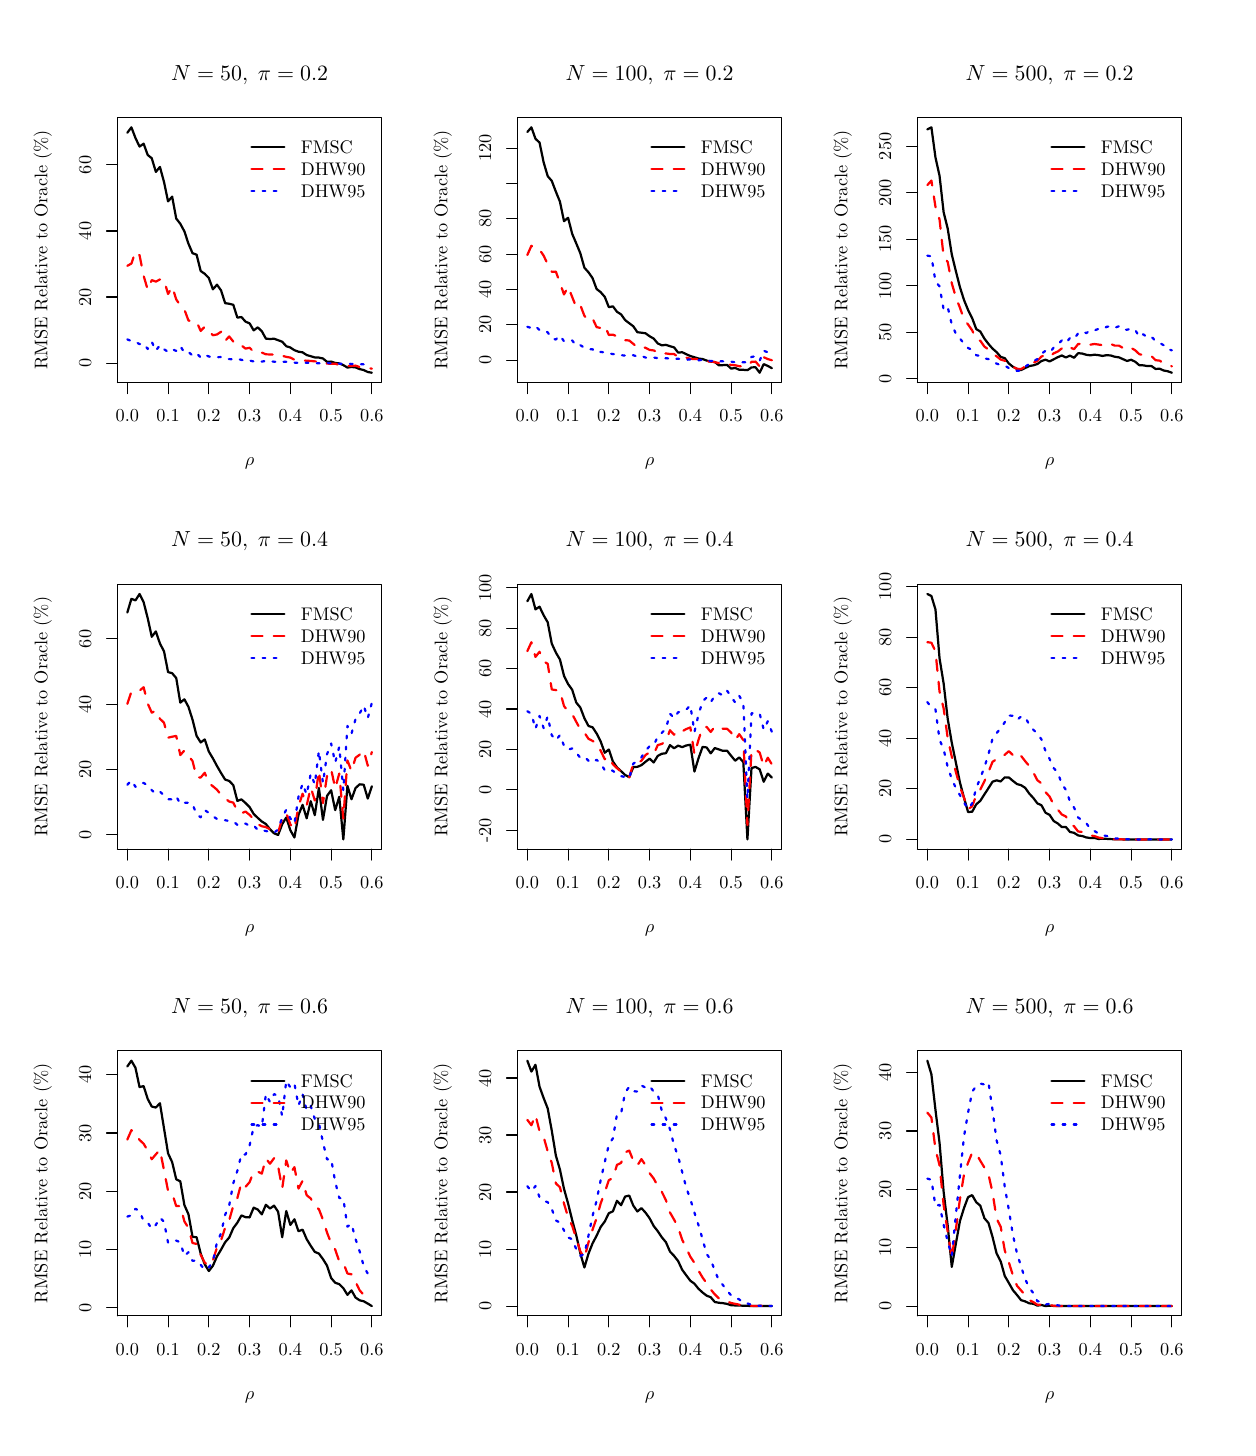
\begin{tikzpicture}[x=1pt,y=1pt]
\definecolor[named]{fillColor}{rgb}{1.00,1.00,1.00}
\path[use as bounding box,fill=fillColor,fill opacity=0.00] (0,0) rectangle (433.62,505.89);
\begin{scope}
\path[clip] ( 32.47,377.65) rectangle (127.91,473.42);
\definecolor[named]{drawColor}{rgb}{0.00,0.00,0.00}

\path[draw=drawColor,line width= 0.8pt,line join=round,line cap=round] ( 36.01,467.91) --
	( 37.48,469.87) --
	( 38.95,466.01) --
	( 40.42,462.92) --
	( 41.90,463.96) --
	( 43.37,459.89) --
	( 44.84,458.69) --
	( 46.32,453.77) --
	( 47.79,455.56) --
	( 49.26,450.15) --
	( 50.73,443.11) --
	( 52.21,444.83) --
	( 53.68,436.90) --
	( 55.15,435.03) --
	( 56.63,432.27) --
	( 58.10,427.83) --
	( 59.57,424.38) --
	( 61.04,423.87) --
	( 62.52,417.95) --
	( 63.99,416.94) --
	( 65.46,415.42) --
	( 66.93,411.34) --
	( 68.41,413.00) --
	( 69.88,410.95) --
	( 71.35,406.34) --
	( 72.83,406.12) --
	( 74.30,405.75) --
	( 75.77,401.11) --
	( 77.24,401.33) --
	( 78.72,399.65) --
	( 80.19,399.04) --
	( 81.66,396.51) --
	( 83.14,397.59) --
	( 84.61,396.19) --
	( 86.08,393.52) --
	( 87.55,393.38) --
	( 89.03,393.49) --
	( 90.50,392.95) --
	( 91.97,392.41) --
	( 93.44,390.79) --
	( 94.92,390.31) --
	( 96.39,389.34) --
	( 97.86,388.80) --
	( 99.34,388.57) --
	(100.81,387.60) --
	(102.28,387.17) --
	(103.75,386.73) --
	(105.23,386.67) --
	(106.70,386.35) --
	(108.17,385.12) --
	(109.65,385.22) --
	(111.12,384.73) --
	(112.59,384.57) --
	(114.06,383.95) --
	(115.54,383.08) --
	(117.01,383.27) --
	(118.48,383.13) --
	(119.95,382.51) --
	(121.43,382.17) --
	(122.90,381.46) --
	(124.37,381.20);
\end{scope}
\begin{scope}
\path[clip] (  0.00,  0.00) rectangle (433.62,505.89);
\definecolor[named]{drawColor}{rgb}{0.00,0.00,0.00}

\path[draw=drawColor,line width= 0.4pt,line join=round,line cap=round] ( 36.01,377.65) -- (124.37,377.65);

\path[draw=drawColor,line width= 0.4pt,line join=round,line cap=round] ( 36.01,377.65) -- ( 36.01,373.69);

\path[draw=drawColor,line width= 0.4pt,line join=round,line cap=round] ( 50.73,377.65) -- ( 50.73,373.69);

\path[draw=drawColor,line width= 0.4pt,line join=round,line cap=round] ( 65.46,377.65) -- ( 65.46,373.69);

\path[draw=drawColor,line width= 0.4pt,line join=round,line cap=round] ( 80.19,377.65) -- ( 80.19,373.69);

\path[draw=drawColor,line width= 0.4pt,line join=round,line cap=round] ( 94.92,377.65) -- ( 94.92,373.69);

\path[draw=drawColor,line width= 0.4pt,line join=round,line cap=round] (109.65,377.65) -- (109.65,373.69);

\path[draw=drawColor,line width= 0.4pt,line join=round,line cap=round] (124.37,377.65) -- (124.37,373.69);

\node[text=drawColor,anchor=base,inner sep=0pt, outer sep=0pt, scale=  0.66] at ( 36.01,363.40) {0.0};

\node[text=drawColor,anchor=base,inner sep=0pt, outer sep=0pt, scale=  0.66] at ( 50.73,363.40) {0.1};

\node[text=drawColor,anchor=base,inner sep=0pt, outer sep=0pt, scale=  0.66] at ( 65.46,363.40) {0.2};

\node[text=drawColor,anchor=base,inner sep=0pt, outer sep=0pt, scale=  0.66] at ( 80.19,363.40) {0.3};

\node[text=drawColor,anchor=base,inner sep=0pt, outer sep=0pt, scale=  0.66] at ( 94.92,363.40) {0.4};

\node[text=drawColor,anchor=base,inner sep=0pt, outer sep=0pt, scale=  0.66] at (109.65,363.40) {0.5};

\node[text=drawColor,anchor=base,inner sep=0pt, outer sep=0pt, scale=  0.66] at (124.37,363.40) {0.6};

\path[draw=drawColor,line width= 0.4pt,line join=round,line cap=round] ( 32.47,384.69) -- ( 32.47,456.30);

\path[draw=drawColor,line width= 0.4pt,line join=round,line cap=round] ( 32.47,384.69) -- ( 28.51,384.69);

\path[draw=drawColor,line width= 0.4pt,line join=round,line cap=round] ( 32.47,408.56) -- ( 28.51,408.56);

\path[draw=drawColor,line width= 0.4pt,line join=round,line cap=round] ( 32.47,432.43) -- ( 28.51,432.43);

\path[draw=drawColor,line width= 0.4pt,line join=round,line cap=round] ( 32.47,456.30) -- ( 28.51,456.30);

\node[text=drawColor,rotate= 90.00,anchor=base,inner sep=0pt, outer sep=0pt, scale=  0.66] at ( 22.97,384.69) {0};

\node[text=drawColor,rotate= 90.00,anchor=base,inner sep=0pt, outer sep=0pt, scale=  0.66] at ( 22.97,408.56) {20};

\node[text=drawColor,rotate= 90.00,anchor=base,inner sep=0pt, outer sep=0pt, scale=  0.66] at ( 22.97,432.43) {40};

\node[text=drawColor,rotate= 90.00,anchor=base,inner sep=0pt, outer sep=0pt, scale=  0.66] at ( 22.97,456.30) {60};

\path[draw=drawColor,line width= 0.4pt,line join=round,line cap=round] ( 32.47,377.65) --
	(127.91,377.65) --
	(127.91,473.42) --
	( 32.47,473.42) --
	( 32.47,377.65);
\end{scope}
\begin{scope}
\path[clip] (  0.00,337.26) rectangle (144.54,505.89);
\definecolor[named]{drawColor}{rgb}{0.00,0.00,0.00}

\node[text=drawColor,anchor=base,inner sep=0pt, outer sep=0pt, scale=  0.79] at ( 80.19,486.92) {\bfseries $N=50, \;\pi=0.2$};

\node[text=drawColor,anchor=base,inner sep=0pt, outer sep=0pt, scale=  0.66] at ( 80.19,347.56) {$\rho$};

\node[text=drawColor,rotate= 90.00,anchor=base,inner sep=0pt, outer sep=0pt, scale=  0.66] at (  7.13,425.53) {RMSE Relative to Oracle (\%)};
\end{scope}
\begin{scope}
\path[clip] ( 32.47,377.65) rectangle (127.91,473.42);
\definecolor[named]{drawColor}{rgb}{1.00,0.00,0.00}

\path[draw=drawColor,line width= 0.8pt,dash pattern=on 4pt off 4pt ,line join=round,line cap=round] ( 36.01,419.82) --
	( 37.48,420.65) --
	( 38.95,424.94) --
	( 40.42,423.67) --
	( 41.90,416.23) --
	( 43.37,411.21) --
	( 44.84,414.67) --
	( 46.32,414.13) --
	( 47.79,414.89) --
	( 49.26,414.71) --
	( 50.73,409.64) --
	( 52.21,412.31) --
	( 53.68,407.71) --
	( 55.15,405.47) --
	( 56.63,404.05) --
	( 58.10,400.05) --
	( 59.57,399.75) --
	( 61.04,399.62) --
	( 62.52,396.30) --
	( 63.99,397.85) --
	( 65.46,396.16) --
	( 66.93,394.75) --
	( 68.41,395.02) --
	( 69.88,396.00) --
	( 71.35,392.72) --
	( 72.83,394.30) --
	( 74.30,392.47) --
	( 75.77,391.01) --
	( 77.24,391.05) --
	( 78.72,389.91) --
	( 80.19,390.22) --
	( 81.66,388.76) --
	( 83.14,388.66) --
	( 84.61,388.48) --
	( 86.08,387.85) --
	( 87.55,387.81) --
	( 89.03,387.74) --
	( 90.50,387.35) --
	( 91.97,387.33) --
	( 93.44,386.93) --
	( 94.92,386.67) --
	( 96.39,385.88) --
	( 97.86,385.65) --
	( 99.34,385.68) --
	(100.81,385.53) --
	(102.28,385.47) --
	(103.75,385.30) --
	(105.23,385.30) --
	(106.70,384.87) --
	(108.17,384.50) --
	(109.65,384.45) --
	(111.12,384.45) --
	(112.59,384.02) --
	(114.06,383.79) --
	(115.54,383.67) --
	(117.01,383.66) --
	(118.48,383.78) --
	(119.95,383.24) --
	(121.43,383.03) --
	(122.90,382.97) --
	(124.37,382.66);
\definecolor[named]{drawColor}{rgb}{0.00,0.00,1.00}

\path[draw=drawColor,line width= 0.8pt,dash pattern=on 1pt off 3pt ,line join=round,line cap=round] ( 36.01,393.26) --
	( 37.48,392.60) --
	( 38.95,392.37) --
	( 40.42,391.54) --
	( 41.90,391.76) --
	( 43.37,389.80) --
	( 44.84,392.37) --
	( 46.32,389.14) --
	( 47.79,391.18) --
	( 49.26,389.68) --
	( 50.73,388.76) --
	( 52.21,389.71) --
	( 53.68,389.08) --
	( 55.15,390.84) --
	( 56.63,388.46) --
	( 58.10,388.71) --
	( 59.57,387.40) --
	( 61.04,388.20) --
	( 62.52,386.70) --
	( 63.99,387.65) --
	( 65.46,387.08) --
	( 66.93,386.71) --
	( 68.41,386.81) --
	( 69.88,386.86) --
	( 71.35,386.31) --
	( 72.83,386.12) --
	( 74.30,386.08) --
	( 75.77,386.23) --
	( 77.24,385.85) --
	( 78.72,385.53) --
	( 80.19,385.62) --
	( 81.66,385.26) --
	( 83.14,385.39) --
	( 84.61,385.22) --
	( 86.08,385.48) --
	( 87.55,385.33) --
	( 89.03,385.19) --
	( 90.50,385.02) --
	( 91.97,385.17) --
	( 93.44,385.13) --
	( 94.92,384.95) --
	( 96.39,384.85) --
	( 97.86,384.76) --
	( 99.34,384.71) --
	(100.81,384.79) --
	(102.28,384.73) --
	(103.75,384.70) --
	(105.23,384.63) --
	(106.70,384.71) --
	(108.17,384.73) --
	(109.65,384.58) --
	(111.12,384.69) --
	(112.59,384.49) --
	(114.06,384.44) --
	(115.54,384.49) --
	(117.01,384.37) --
	(118.48,384.38) --
	(119.95,384.30) --
	(121.43,384.22) --
	(122.90,384.18) --
	(124.37,384.12);
\definecolor[named]{drawColor}{rgb}{0.00,0.00,0.00}

\path[draw=drawColor,line width= 0.8pt,line join=round,line cap=round] ( 80.89,462.63) -- ( 92.77,462.63);
\definecolor[named]{drawColor}{rgb}{1.00,0.00,0.00}

\path[draw=drawColor,line width= 0.8pt,dash pattern=on 4pt off 4pt ,line join=round,line cap=round] ( 80.89,454.71) -- ( 92.77,454.71);
\definecolor[named]{drawColor}{rgb}{0.00,0.00,1.00}

\path[draw=drawColor,line width= 0.8pt,dash pattern=on 1pt off 3pt ,line join=round,line cap=round] ( 80.89,446.79) -- ( 92.77,446.79);
\definecolor[named]{drawColor}{rgb}{0.00,0.00,0.00}

\node[text=drawColor,anchor=base west,inner sep=0pt, outer sep=0pt, scale=  0.66] at ( 98.71,460.35) {FMSC};

\node[text=drawColor,anchor=base west,inner sep=0pt, outer sep=0pt, scale=  0.66] at ( 98.71,452.43) {DHW90};

\node[text=drawColor,anchor=base west,inner sep=0pt, outer sep=0pt, scale=  0.66] at ( 98.71,444.51) {DHW95};
\end{scope}
\begin{scope}
\path[clip] (177.01,377.65) rectangle (272.45,473.42);
\definecolor[named]{drawColor}{rgb}{0.00,0.00,0.00}

\path[draw=drawColor,line width= 0.8pt,line join=round,line cap=round] (180.55,468.19) --
	(182.02,469.87) --
	(183.49,465.74) --
	(184.96,464.37) --
	(186.44,457.24) --
	(187.91,452.23) --
	(189.38,450.52) --
	(190.86,446.63) --
	(192.33,443.01) --
	(193.80,435.96) --
	(195.27,437.19) --
	(196.75,431.41) --
	(198.22,427.95) --
	(199.69,424.40) --
	(201.17,419.14) --
	(202.64,417.50) --
	(204.11,415.40) --
	(205.58,411.45) --
	(207.06,410.30) --
	(208.53,408.61) --
	(210.00,404.88) --
	(211.47,405.19) --
	(212.95,403.21) --
	(214.42,402.29) --
	(215.89,400.22) --
	(217.37,399.09) --
	(218.84,397.99) --
	(220.31,395.84) --
	(221.78,395.66) --
	(223.26,395.46) --
	(224.73,394.38) --
	(226.20,393.54) --
	(227.68,391.79) --
	(229.15,391.09) --
	(230.62,391.28) --
	(232.09,390.78) --
	(233.57,390.37) --
	(235.04,388.47) --
	(236.51,388.60) --
	(237.98,387.90) --
	(239.46,387.23) --
	(240.93,386.79) --
	(242.40,386.33) --
	(243.88,386.14) --
	(245.35,385.59) --
	(246.82,385.21) --
	(248.29,385.08) --
	(249.77,383.86) --
	(251.24,383.94) --
	(252.71,384.04) --
	(254.19,382.69) --
	(255.66,382.93) --
	(257.13,382.27) --
	(258.60,382.25) --
	(260.08,382.13) --
	(261.55,383.12) --
	(263.02,383.17) --
	(264.50,381.20) --
	(265.97,384.31) --
	(267.44,383.65) --
	(268.91,382.85);
\end{scope}
\begin{scope}
\path[clip] (  0.00,  0.00) rectangle (433.62,505.89);
\definecolor[named]{drawColor}{rgb}{0.00,0.00,0.00}

\path[draw=drawColor,line width= 0.4pt,line join=round,line cap=round] (180.55,377.65) -- (268.91,377.65);

\path[draw=drawColor,line width= 0.4pt,line join=round,line cap=round] (180.55,377.65) -- (180.55,373.69);

\path[draw=drawColor,line width= 0.4pt,line join=round,line cap=round] (195.27,377.65) -- (195.27,373.69);

\path[draw=drawColor,line width= 0.4pt,line join=round,line cap=round] (210.00,377.65) -- (210.00,373.69);

\path[draw=drawColor,line width= 0.4pt,line join=round,line cap=round] (224.73,377.65) -- (224.73,373.69);

\path[draw=drawColor,line width= 0.4pt,line join=round,line cap=round] (239.46,377.65) -- (239.46,373.69);

\path[draw=drawColor,line width= 0.4pt,line join=round,line cap=round] (254.19,377.65) -- (254.19,373.69);

\path[draw=drawColor,line width= 0.4pt,line join=round,line cap=round] (268.91,377.65) -- (268.91,373.69);

\node[text=drawColor,anchor=base,inner sep=0pt, outer sep=0pt, scale=  0.66] at (180.55,363.40) {0.0};

\node[text=drawColor,anchor=base,inner sep=0pt, outer sep=0pt, scale=  0.66] at (195.27,363.40) {0.1};

\node[text=drawColor,anchor=base,inner sep=0pt, outer sep=0pt, scale=  0.66] at (210.00,363.40) {0.2};

\node[text=drawColor,anchor=base,inner sep=0pt, outer sep=0pt, scale=  0.66] at (224.73,363.40) {0.3};

\node[text=drawColor,anchor=base,inner sep=0pt, outer sep=0pt, scale=  0.66] at (239.46,363.40) {0.4};

\node[text=drawColor,anchor=base,inner sep=0pt, outer sep=0pt, scale=  0.66] at (254.19,363.40) {0.5};

\node[text=drawColor,anchor=base,inner sep=0pt, outer sep=0pt, scale=  0.66] at (268.91,363.40) {0.6};

\path[draw=drawColor,line width= 0.4pt,line join=round,line cap=round] (177.01,385.73) -- (177.01,462.35);

\path[draw=drawColor,line width= 0.4pt,line join=round,line cap=round] (177.01,385.73) -- (173.05,385.73);

\path[draw=drawColor,line width= 0.4pt,line join=round,line cap=round] (177.01,398.50) -- (173.05,398.50);

\path[draw=drawColor,line width= 0.4pt,line join=round,line cap=round] (177.01,411.27) -- (173.05,411.27);

\path[draw=drawColor,line width= 0.4pt,line join=round,line cap=round] (177.01,424.04) -- (173.05,424.04);

\path[draw=drawColor,line width= 0.4pt,line join=round,line cap=round] (177.01,436.81) -- (173.05,436.81);

\path[draw=drawColor,line width= 0.4pt,line join=round,line cap=round] (177.01,449.58) -- (173.05,449.58);

\path[draw=drawColor,line width= 0.4pt,line join=round,line cap=round] (177.01,462.35) -- (173.05,462.35);

\node[text=drawColor,rotate= 90.00,anchor=base,inner sep=0pt, outer sep=0pt, scale=  0.66] at (167.51,385.73) {0};

\node[text=drawColor,rotate= 90.00,anchor=base,inner sep=0pt, outer sep=0pt, scale=  0.66] at (167.51,398.50) {20};

\node[text=drawColor,rotate= 90.00,anchor=base,inner sep=0pt, outer sep=0pt, scale=  0.66] at (167.51,411.27) {40};

\node[text=drawColor,rotate= 90.00,anchor=base,inner sep=0pt, outer sep=0pt, scale=  0.66] at (167.51,424.04) {60};

\node[text=drawColor,rotate= 90.00,anchor=base,inner sep=0pt, outer sep=0pt, scale=  0.66] at (167.51,436.81) {80};

\node[text=drawColor,rotate= 90.00,anchor=base,inner sep=0pt, outer sep=0pt, scale=  0.66] at (167.51,462.35) {120};

\path[draw=drawColor,line width= 0.4pt,line join=round,line cap=round] (177.01,377.65) --
	(272.45,377.65) --
	(272.45,473.42) --
	(177.01,473.42) --
	(177.01,377.65);
\end{scope}
\begin{scope}
\path[clip] (144.54,337.26) rectangle (289.08,505.89);
\definecolor[named]{drawColor}{rgb}{0.00,0.00,0.00}

\node[text=drawColor,anchor=base,inner sep=0pt, outer sep=0pt, scale=  0.79] at (224.73,486.92) {\bfseries $N=100, \;\pi=0.2$};

\node[text=drawColor,anchor=base,inner sep=0pt, outer sep=0pt, scale=  0.66] at (224.73,347.56) {$\rho$};

\node[text=drawColor,rotate= 90.00,anchor=base,inner sep=0pt, outer sep=0pt, scale=  0.66] at (151.67,425.53) {RMSE Relative to Oracle (\%)};
\end{scope}
\begin{scope}
\path[clip] (177.01,377.65) rectangle (272.45,473.42);
\definecolor[named]{drawColor}{rgb}{1.00,0.00,0.00}

\path[draw=drawColor,line width= 0.8pt,dash pattern=on 4pt off 4pt ,line join=round,line cap=round] (180.55,423.74) --
	(182.02,427.07) --
	(183.49,425.81) --
	(184.96,425.67) --
	(186.44,423.53) --
	(187.91,420.36) --
	(189.38,417.68) --
	(190.86,417.74) --
	(192.33,413.66) --
	(193.80,409.48) --
	(195.27,412.29) --
	(196.75,408.60) --
	(198.22,404.84) --
	(199.69,405.65) --
	(201.17,401.76) --
	(202.64,400.18) --
	(204.11,400.83) --
	(205.58,397.69) --
	(207.06,397.35) --
	(208.53,398.21) --
	(210.00,394.85) --
	(211.47,394.95) --
	(212.95,394.34) --
	(214.42,393.35) --
	(215.89,392.97) --
	(217.37,392.84) --
	(218.84,391.62) --
	(220.31,390.42) --
	(221.78,390.73) --
	(223.26,390.19) --
	(224.73,389.44) --
	(226.20,389.26) --
	(227.68,388.57) --
	(229.15,387.96) --
	(230.62,388.17) --
	(232.09,387.97) --
	(233.57,387.96) --
	(235.04,386.92) --
	(236.51,386.90) --
	(237.98,386.69) --
	(239.46,386.23) --
	(240.93,386.16) --
	(242.40,386.09) --
	(243.88,385.86) --
	(245.35,385.29) --
	(246.82,385.29) --
	(248.29,385.01) --
	(249.77,384.69) --
	(251.24,384.63) --
	(252.71,384.53) --
	(254.19,384.00) --
	(255.66,383.89) --
	(257.13,383.56) --
	(258.60,383.47) --
	(260.08,383.68) --
	(261.55,385.14) --
	(263.02,385.22) --
	(264.50,383.47) --
	(265.97,386.82) --
	(267.44,386.13) --
	(268.91,385.72);
\definecolor[named]{drawColor}{rgb}{0.00,0.00,1.00}

\path[draw=drawColor,line width= 0.8pt,dash pattern=on 1pt off 3pt ,line join=round,line cap=round] (180.55,397.79) --
	(182.02,397.37) --
	(183.49,397.97) --
	(184.96,396.62) --
	(186.44,396.68) --
	(187.91,395.78) --
	(189.38,393.58) --
	(190.86,393.21) --
	(192.33,394.66) --
	(193.80,392.57) --
	(195.27,392.78) --
	(196.75,392.87) --
	(198.22,390.96) --
	(199.69,391.16) --
	(201.17,390.24) --
	(202.64,389.71) --
	(204.11,389.66) --
	(205.58,388.47) --
	(207.06,388.74) --
	(208.53,388.49) --
	(210.00,388.22) --
	(211.47,387.91) --
	(212.95,388.01) --
	(214.42,387.51) --
	(215.89,387.42) --
	(217.37,387.78) --
	(218.84,387.52) --
	(220.31,387.03) --
	(221.78,387.26) --
	(223.26,386.68) --
	(224.73,386.47) --
	(226.20,386.69) --
	(227.68,386.48) --
	(229.15,386.38) --
	(230.62,386.44) --
	(232.09,386.32) --
	(233.57,386.20) --
	(235.04,386.23) --
	(236.51,386.20) --
	(237.98,385.90) --
	(239.46,385.99) --
	(240.93,385.89) --
	(242.40,385.71) --
	(243.88,385.80) --
	(245.35,385.54) --
	(246.82,385.47) --
	(248.29,385.36) --
	(249.77,385.33) --
	(251.24,385.31) --
	(252.71,385.32) --
	(254.19,385.18) --
	(255.66,384.98) --
	(257.13,384.95) --
	(258.60,384.99) --
	(260.08,384.97) --
	(261.55,386.91) --
	(263.02,387.15) --
	(264.50,385.55) --
	(265.97,389.13) --
	(267.44,388.59) --
	(268.91,388.44);
\definecolor[named]{drawColor}{rgb}{0.00,0.00,0.00}

\path[draw=drawColor,line width= 0.8pt,line join=round,line cap=round] (225.43,462.63) -- (237.31,462.63);
\definecolor[named]{drawColor}{rgb}{1.00,0.00,0.00}

\path[draw=drawColor,line width= 0.8pt,dash pattern=on 4pt off 4pt ,line join=round,line cap=round] (225.43,454.71) -- (237.31,454.71);
\definecolor[named]{drawColor}{rgb}{0.00,0.00,1.00}

\path[draw=drawColor,line width= 0.8pt,dash pattern=on 1pt off 3pt ,line join=round,line cap=round] (225.43,446.79) -- (237.31,446.79);
\definecolor[named]{drawColor}{rgb}{0.00,0.00,0.00}

\node[text=drawColor,anchor=base west,inner sep=0pt, outer sep=0pt, scale=  0.66] at (243.25,460.35) {FMSC};

\node[text=drawColor,anchor=base west,inner sep=0pt, outer sep=0pt, scale=  0.66] at (243.25,452.43) {DHW90};

\node[text=drawColor,anchor=base west,inner sep=0pt, outer sep=0pt, scale=  0.66] at (243.25,444.51) {DHW95};
\end{scope}
\begin{scope}
\path[clip] (321.55,377.65) rectangle (416.99,473.42);
\definecolor[named]{drawColor}{rgb}{0.00,0.00,0.00}

\path[draw=drawColor,line width= 0.8pt,line join=round,line cap=round] (325.09,469.12) --
	(326.56,469.87) --
	(328.03,458.97) --
	(329.50,452.39) --
	(330.98,439.19) --
	(332.45,433.27) --
	(333.92,423.97) --
	(335.40,417.89) --
	(336.87,412.12) --
	(338.34,407.48) --
	(339.81,403.89) --
	(341.29,400.93) --
	(342.76,396.98) --
	(344.23,396.08) --
	(345.71,393.53) --
	(347.18,391.61) --
	(348.65,389.91) --
	(350.12,388.64) --
	(351.60,386.93) --
	(353.07,386.46) --
	(354.54,384.54) --
	(356.01,383.34) --
	(357.49,382.56) --
	(358.96,382.15) --
	(360.43,382.89) --
	(361.91,383.61) --
	(363.38,383.87) --
	(364.85,384.34) --
	(366.32,385.43) --
	(367.80,385.91) --
	(369.27,385.28) --
	(370.74,386.05) --
	(372.22,386.81) --
	(373.69,387.44) --
	(375.16,386.71) --
	(376.63,387.39) --
	(378.11,386.60) --
	(379.58,388.26) --
	(381.05,388.13) --
	(382.52,387.68) --
	(384.00,387.49) --
	(385.47,387.71) --
	(386.94,387.55) --
	(388.42,387.27) --
	(389.89,387.55) --
	(391.36,387.43) --
	(392.83,386.97) --
	(394.31,386.76) --
	(395.78,386.11) --
	(397.25,385.45) --
	(398.73,385.89) --
	(400.20,385.18) --
	(401.67,383.92) --
	(403.14,383.86) --
	(404.62,383.60) --
	(406.09,383.61) --
	(407.56,382.56) --
	(409.04,382.65) --
	(410.51,382.00) --
	(411.98,381.73) --
	(413.45,381.20);
\end{scope}
\begin{scope}
\path[clip] (  0.00,  0.00) rectangle (433.62,505.89);
\definecolor[named]{drawColor}{rgb}{0.00,0.00,0.00}

\path[draw=drawColor,line width= 0.4pt,line join=round,line cap=round] (325.09,377.65) -- (413.45,377.65);

\path[draw=drawColor,line width= 0.4pt,line join=round,line cap=round] (325.09,377.65) -- (325.09,373.69);

\path[draw=drawColor,line width= 0.4pt,line join=round,line cap=round] (339.81,377.65) -- (339.81,373.69);

\path[draw=drawColor,line width= 0.4pt,line join=round,line cap=round] (354.54,377.65) -- (354.54,373.69);

\path[draw=drawColor,line width= 0.4pt,line join=round,line cap=round] (369.27,377.65) -- (369.27,373.69);

\path[draw=drawColor,line width= 0.4pt,line join=round,line cap=round] (384.00,377.65) -- (384.00,373.69);

\path[draw=drawColor,line width= 0.4pt,line join=round,line cap=round] (398.73,377.65) -- (398.73,373.69);

\path[draw=drawColor,line width= 0.4pt,line join=round,line cap=round] (413.45,377.65) -- (413.45,373.69);

\node[text=drawColor,anchor=base,inner sep=0pt, outer sep=0pt, scale=  0.66] at (325.09,363.40) {0.0};

\node[text=drawColor,anchor=base,inner sep=0pt, outer sep=0pt, scale=  0.66] at (339.81,363.40) {0.1};

\node[text=drawColor,anchor=base,inner sep=0pt, outer sep=0pt, scale=  0.66] at (354.54,363.40) {0.2};

\node[text=drawColor,anchor=base,inner sep=0pt, outer sep=0pt, scale=  0.66] at (369.27,363.40) {0.3};

\node[text=drawColor,anchor=base,inner sep=0pt, outer sep=0pt, scale=  0.66] at (384.00,363.40) {0.4};

\node[text=drawColor,anchor=base,inner sep=0pt, outer sep=0pt, scale=  0.66] at (398.73,363.40) {0.5};

\node[text=drawColor,anchor=base,inner sep=0pt, outer sep=0pt, scale=  0.66] at (413.45,363.40) {0.6};

\path[draw=drawColor,line width= 0.4pt,line join=round,line cap=round] (321.55,379.06) -- (321.55,463.01);

\path[draw=drawColor,line width= 0.4pt,line join=round,line cap=round] (321.55,379.06) -- (317.59,379.06);

\path[draw=drawColor,line width= 0.4pt,line join=round,line cap=round] (321.55,395.85) -- (317.59,395.85);

\path[draw=drawColor,line width= 0.4pt,line join=round,line cap=round] (321.55,412.64) -- (317.59,412.64);

\path[draw=drawColor,line width= 0.4pt,line join=round,line cap=round] (321.55,429.43) -- (317.59,429.43);

\path[draw=drawColor,line width= 0.4pt,line join=round,line cap=round] (321.55,446.22) -- (317.59,446.22);

\path[draw=drawColor,line width= 0.4pt,line join=round,line cap=round] (321.55,463.01) -- (317.59,463.01);

\node[text=drawColor,rotate= 90.00,anchor=base,inner sep=0pt, outer sep=0pt, scale=  0.66] at (312.05,379.06) {0};

\node[text=drawColor,rotate= 90.00,anchor=base,inner sep=0pt, outer sep=0pt, scale=  0.66] at (312.05,395.85) {50};

\node[text=drawColor,rotate= 90.00,anchor=base,inner sep=0pt, outer sep=0pt, scale=  0.66] at (312.05,412.64) {100};

\node[text=drawColor,rotate= 90.00,anchor=base,inner sep=0pt, outer sep=0pt, scale=  0.66] at (312.05,429.43) {150};

\node[text=drawColor,rotate= 90.00,anchor=base,inner sep=0pt, outer sep=0pt, scale=  0.66] at (312.05,446.22) {200};

\node[text=drawColor,rotate= 90.00,anchor=base,inner sep=0pt, outer sep=0pt, scale=  0.66] at (312.05,463.01) {250};

\path[draw=drawColor,line width= 0.4pt,line join=round,line cap=round] (321.55,377.65) --
	(416.99,377.65) --
	(416.99,473.42) --
	(321.55,473.42) --
	(321.55,377.65);
\end{scope}
\begin{scope}
\path[clip] (289.08,337.26) rectangle (433.62,505.89);
\definecolor[named]{drawColor}{rgb}{0.00,0.00,0.00}

\node[text=drawColor,anchor=base,inner sep=0pt, outer sep=0pt, scale=  0.79] at (369.27,486.92) {\bfseries $N=500, \;\pi=0.2$};

\node[text=drawColor,anchor=base,inner sep=0pt, outer sep=0pt, scale=  0.66] at (369.27,347.56) {$\rho$};

\node[text=drawColor,rotate= 90.00,anchor=base,inner sep=0pt, outer sep=0pt, scale=  0.66] at (296.21,425.53) {RMSE Relative to Oracle (\%)};
\end{scope}
\begin{scope}
\path[clip] (321.55,377.65) rectangle (416.99,473.42);
\definecolor[named]{drawColor}{rgb}{1.00,0.00,0.00}

\path[draw=drawColor,line width= 0.8pt,dash pattern=on 4pt off 4pt ,line join=round,line cap=round] (325.09,448.99) --
	(326.56,450.64) --
	(328.03,441.14) --
	(329.50,436.55) --
	(330.98,423.09) --
	(332.45,421.24) --
	(333.92,413.53) --
	(335.40,408.46) --
	(336.87,404.68) --
	(338.34,400.52) --
	(339.81,398.63) --
	(341.29,396.51) --
	(342.76,393.32) --
	(344.23,392.75) --
	(345.71,390.64) --
	(347.18,389.60) --
	(348.65,388.17) --
	(350.12,387.13) --
	(351.60,385.96) --
	(353.07,385.51) --
	(354.54,384.19) --
	(356.01,383.31) --
	(357.49,382.64) --
	(358.96,382.49) --
	(360.43,383.44) --
	(361.91,384.27) --
	(363.38,384.79) --
	(364.85,385.48) --
	(366.32,387.04) --
	(367.80,387.61) --
	(369.27,386.98) --
	(370.74,388.20) --
	(372.22,388.86) --
	(373.69,389.99) --
	(375.16,389.24) --
	(376.63,390.32) --
	(378.11,389.72) --
	(379.58,391.57) --
	(381.05,391.67) --
	(382.52,391.09) --
	(384.00,391.33) --
	(385.47,391.58) --
	(386.94,391.38) --
	(388.42,391.15) --
	(389.89,391.74) --
	(391.36,391.58) --
	(392.83,390.99) --
	(394.31,390.99) --
	(395.78,390.15) --
	(397.25,389.51) --
	(398.73,390.16) --
	(400.20,389.31) --
	(401.67,387.91) --
	(403.14,387.54) --
	(404.62,387.10) --
	(406.09,387.21) --
	(407.56,385.72) --
	(409.04,385.57) --
	(410.51,384.59) --
	(411.98,384.02) --
	(413.45,383.51);
\definecolor[named]{drawColor}{rgb}{0.00,0.00,1.00}

\path[draw=drawColor,line width= 0.8pt,dash pattern=on 1pt off 3pt ,line join=round,line cap=round] (325.09,423.51) --
	(326.56,423.26) --
	(328.03,414.15) --
	(329.50,412.41) --
	(330.98,404.02) --
	(332.45,404.93) --
	(333.92,398.67) --
	(335.40,395.30) --
	(336.87,393.58) --
	(338.34,391.67) --
	(339.81,390.14) --
	(341.29,389.43) --
	(342.76,387.53) --
	(344.23,387.24) --
	(345.71,386.36) --
	(347.18,386.12) --
	(348.65,385.11) --
	(350.12,384.51) --
	(351.60,383.95) --
	(353.07,383.75) --
	(354.54,382.88) --
	(356.01,382.60) --
	(357.49,381.86) --
	(358.96,381.99) --
	(360.43,383.33) --
	(361.91,384.39) --
	(363.38,385.38) --
	(364.85,386.12) --
	(366.32,388.07) --
	(367.80,389.12) --
	(369.27,388.53) --
	(370.74,390.26) --
	(372.22,391.30) --
	(373.69,392.92) --
	(375.16,391.96) --
	(376.63,393.74) --
	(378.11,393.35) --
	(379.58,395.45) --
	(381.05,396.13) --
	(382.52,395.53) --
	(384.00,396.50) --
	(385.47,396.48) --
	(386.94,397.05) --
	(388.42,396.88) --
	(389.89,397.79) --
	(391.36,398.02) --
	(392.83,397.45) --
	(394.31,397.99) --
	(395.78,396.86) --
	(397.25,396.74) --
	(398.73,397.13) --
	(400.20,396.73) --
	(401.67,394.10) --
	(403.14,395.08) --
	(404.62,393.88) --
	(406.09,394.18) --
	(407.56,392.70) --
	(409.04,392.00) --
	(410.51,391.11) --
	(411.98,389.71) --
	(413.45,389.30);
\definecolor[named]{drawColor}{rgb}{0.00,0.00,0.00}

\path[draw=drawColor,line width= 0.8pt,line join=round,line cap=round] (369.97,462.63) -- (381.85,462.63);
\definecolor[named]{drawColor}{rgb}{1.00,0.00,0.00}

\path[draw=drawColor,line width= 0.8pt,dash pattern=on 4pt off 4pt ,line join=round,line cap=round] (369.97,454.71) -- (381.85,454.71);
\definecolor[named]{drawColor}{rgb}{0.00,0.00,1.00}

\path[draw=drawColor,line width= 0.8pt,dash pattern=on 1pt off 3pt ,line join=round,line cap=round] (369.97,446.79) -- (381.85,446.79);
\definecolor[named]{drawColor}{rgb}{0.00,0.00,0.00}

\node[text=drawColor,anchor=base west,inner sep=0pt, outer sep=0pt, scale=  0.66] at (387.79,460.35) {FMSC};

\node[text=drawColor,anchor=base west,inner sep=0pt, outer sep=0pt, scale=  0.66] at (387.79,452.43) {DHW90};

\node[text=drawColor,anchor=base west,inner sep=0pt, outer sep=0pt, scale=  0.66] at (387.79,444.51) {DHW95};
\end{scope}
\begin{scope}
\path[clip] ( 32.47,209.02) rectangle (127.91,304.79);
\definecolor[named]{drawColor}{rgb}{0.00,0.00,0.00}

\path[draw=drawColor,line width= 0.8pt,line join=round,line cap=round] ( 36.01,294.56) --
	( 37.48,299.51) --
	( 38.95,298.93) --
	( 40.42,301.24) --
	( 41.90,298.28) --
	( 43.37,292.52) --
	( 44.84,285.79) --
	( 46.32,287.72) --
	( 47.79,283.35) --
	( 49.26,280.55) --
	( 50.73,273.03) --
	( 52.21,272.62) --
	( 53.68,270.86) --
	( 55.15,261.99) --
	( 56.63,263.19) --
	( 58.10,260.46) --
	( 59.57,255.83) --
	( 61.04,249.97) --
	( 62.52,247.61) --
	( 63.99,248.69) --
	( 65.46,244.31) --
	( 66.93,241.85) --
	( 68.41,239.10) --
	( 69.88,236.55) --
	( 71.35,234.18) --
	( 72.83,233.69) --
	( 74.30,232.17) --
	( 75.77,226.47) --
	( 77.24,227.03) --
	( 78.72,225.72) --
	( 80.19,224.25) --
	( 81.66,221.77) --
	( 83.14,220.34) --
	( 84.61,219.03) --
	( 86.08,218.13) --
	( 87.55,216.26) --
	( 89.03,214.77) --
	( 90.50,214.17) --
	( 91.97,218.06) --
	( 93.44,220.49) --
	( 94.92,215.88) --
	( 96.39,213.26) --
	( 97.86,221.44) --
	( 99.34,225.06) --
	(100.81,220.19) --
	(102.28,226.36) --
	(103.75,221.33) --
	(105.23,231.19) --
	(106.70,219.62) --
	(108.17,228.29) --
	(109.65,230.33) --
	(111.12,223.14) --
	(112.59,227.95) --
	(114.06,212.57) --
	(115.54,231.92) --
	(117.01,227.07) --
	(118.48,231.12) --
	(119.95,232.48) --
	(121.43,232.32) --
	(122.90,227.32) --
	(124.37,231.78);
\end{scope}
\begin{scope}
\path[clip] (  0.00,  0.00) rectangle (433.62,505.89);
\definecolor[named]{drawColor}{rgb}{0.00,0.00,0.00}

\path[draw=drawColor,line width= 0.4pt,line join=round,line cap=round] ( 36.01,209.02) -- (124.37,209.02);

\path[draw=drawColor,line width= 0.4pt,line join=round,line cap=round] ( 36.01,209.02) -- ( 36.01,205.06);

\path[draw=drawColor,line width= 0.4pt,line join=round,line cap=round] ( 50.73,209.02) -- ( 50.73,205.06);

\path[draw=drawColor,line width= 0.4pt,line join=round,line cap=round] ( 65.46,209.02) -- ( 65.46,205.06);

\path[draw=drawColor,line width= 0.4pt,line join=round,line cap=round] ( 80.19,209.02) -- ( 80.19,205.06);

\path[draw=drawColor,line width= 0.4pt,line join=round,line cap=round] ( 94.92,209.02) -- ( 94.92,205.06);

\path[draw=drawColor,line width= 0.4pt,line join=round,line cap=round] (109.65,209.02) -- (109.65,205.06);

\path[draw=drawColor,line width= 0.4pt,line join=round,line cap=round] (124.37,209.02) -- (124.37,205.06);

\node[text=drawColor,anchor=base,inner sep=0pt, outer sep=0pt, scale=  0.66] at ( 36.01,194.77) {0.0};

\node[text=drawColor,anchor=base,inner sep=0pt, outer sep=0pt, scale=  0.66] at ( 50.73,194.77) {0.1};

\node[text=drawColor,anchor=base,inner sep=0pt, outer sep=0pt, scale=  0.66] at ( 65.46,194.77) {0.2};

\node[text=drawColor,anchor=base,inner sep=0pt, outer sep=0pt, scale=  0.66] at ( 80.19,194.77) {0.3};

\node[text=drawColor,anchor=base,inner sep=0pt, outer sep=0pt, scale=  0.66] at ( 94.92,194.77) {0.4};

\node[text=drawColor,anchor=base,inner sep=0pt, outer sep=0pt, scale=  0.66] at (109.65,194.77) {0.5};

\node[text=drawColor,anchor=base,inner sep=0pt, outer sep=0pt, scale=  0.66] at (124.37,194.77) {0.6};

\path[draw=drawColor,line width= 0.4pt,line join=round,line cap=round] ( 32.47,214.26) -- ( 32.47,285.03);

\path[draw=drawColor,line width= 0.4pt,line join=round,line cap=round] ( 32.47,214.26) -- ( 28.51,214.26);

\path[draw=drawColor,line width= 0.4pt,line join=round,line cap=round] ( 32.47,237.85) -- ( 28.51,237.85);

\path[draw=drawColor,line width= 0.4pt,line join=round,line cap=round] ( 32.47,261.44) -- ( 28.51,261.44);

\path[draw=drawColor,line width= 0.4pt,line join=round,line cap=round] ( 32.47,285.03) -- ( 28.51,285.03);

\node[text=drawColor,rotate= 90.00,anchor=base,inner sep=0pt, outer sep=0pt, scale=  0.66] at ( 22.97,214.26) {0};

\node[text=drawColor,rotate= 90.00,anchor=base,inner sep=0pt, outer sep=0pt, scale=  0.66] at ( 22.97,237.85) {20};

\node[text=drawColor,rotate= 90.00,anchor=base,inner sep=0pt, outer sep=0pt, scale=  0.66] at ( 22.97,261.44) {40};

\node[text=drawColor,rotate= 90.00,anchor=base,inner sep=0pt, outer sep=0pt, scale=  0.66] at ( 22.97,285.03) {60};

\path[draw=drawColor,line width= 0.4pt,line join=round,line cap=round] ( 32.47,209.02) --
	(127.91,209.02) --
	(127.91,304.79) --
	( 32.47,304.79) --
	( 32.47,209.02);
\end{scope}
\begin{scope}
\path[clip] (  0.00,168.63) rectangle (144.54,337.26);
\definecolor[named]{drawColor}{rgb}{0.00,0.00,0.00}

\node[text=drawColor,anchor=base,inner sep=0pt, outer sep=0pt, scale=  0.79] at ( 80.19,318.29) {\bfseries $N=50, \;\pi=0.4$};

\node[text=drawColor,anchor=base,inner sep=0pt, outer sep=0pt, scale=  0.66] at ( 80.19,178.93) {$\rho$};

\node[text=drawColor,rotate= 90.00,anchor=base,inner sep=0pt, outer sep=0pt, scale=  0.66] at (  7.13,256.90) {RMSE Relative to Oracle (\%)};
\end{scope}
\begin{scope}
\path[clip] ( 32.47,209.02) rectangle (127.91,304.79);
\definecolor[named]{drawColor}{rgb}{1.00,0.00,0.00}

\path[draw=drawColor,line width= 0.8pt,dash pattern=on 4pt off 4pt ,line join=round,line cap=round] ( 36.01,261.53) --
	( 37.48,265.99) --
	( 38.95,266.18) --
	( 40.42,266.34) --
	( 41.90,267.55) --
	( 43.37,261.67) --
	( 44.84,258.36) --
	( 46.32,259.13) --
	( 47.79,256.15) --
	( 49.26,254.73) --
	( 50.73,249.32) --
	( 52.21,249.68) --
	( 53.68,249.96) --
	( 55.15,243.03) --
	( 56.63,244.71) --
	( 58.10,242.78) --
	( 59.57,240.90) --
	( 61.04,235.04) --
	( 62.52,234.93) --
	( 63.99,236.65) --
	( 65.46,232.81) --
	( 66.93,231.79) --
	( 68.41,230.52) --
	( 69.88,228.66) --
	( 71.35,227.36) --
	( 72.83,226.25) --
	( 74.30,225.86) --
	( 75.77,222.87) --
	( 77.24,222.02) --
	( 78.72,222.62) --
	( 80.19,221.44) --
	( 81.66,219.88) --
	( 83.14,218.05) --
	( 84.61,217.32) --
	( 86.08,217.02) --
	( 87.55,216.25) --
	( 89.03,215.50) --
	( 90.50,215.08) --
	( 91.97,220.03) --
	( 93.44,222.14) --
	( 94.92,218.00) --
	( 96.39,216.24) --
	( 97.86,224.55) --
	( 99.34,229.08) --
	(100.81,224.75) --
	(102.28,231.40) --
	(103.75,226.63) --
	(105.23,237.38) --
	(106.70,225.68) --
	(108.17,235.56) --
	(109.65,238.00) --
	(111.12,231.00) --
	(112.59,236.36) --
	(114.06,220.11) --
	(115.54,241.10) --
	(117.01,237.29) --
	(118.48,242.08) --
	(119.95,243.16) --
	(121.43,244.71) --
	(122.90,239.20) --
	(124.37,244.15);
\definecolor[named]{drawColor}{rgb}{0.00,0.00,1.00}

\path[draw=drawColor,line width= 0.8pt,dash pattern=on 1pt off 3pt ,line join=round,line cap=round] ( 36.01,232.32) --
	( 37.48,233.87) --
	( 38.95,231.59) --
	( 40.42,232.79) --
	( 41.90,232.97) --
	( 43.37,232.09) --
	( 44.84,230.35) --
	( 46.32,229.08) --
	( 47.79,229.81) --
	( 49.26,228.50) --
	( 50.73,227.09) --
	( 52.21,227.02) --
	( 53.68,228.13) --
	( 55.15,225.39) --
	( 56.63,225.81) --
	( 58.10,225.82) --
	( 59.57,225.32) --
	( 61.04,221.57) --
	( 62.52,220.57) --
	( 63.99,223.16) --
	( 65.46,222.13) --
	( 66.93,220.94) --
	( 68.41,219.96) --
	( 69.88,219.47) --
	( 71.35,219.49) --
	( 72.83,219.21) --
	( 74.30,219.07) --
	( 75.77,217.83) --
	( 77.24,217.57) --
	( 78.72,218.32) --
	( 80.19,217.41) --
	( 81.66,217.60) --
	( 83.14,216.02) --
	( 84.61,215.78) --
	( 86.08,215.63) --
	( 87.55,215.16) --
	( 89.03,214.99) --
	( 90.50,216.13) --
	( 91.97,220.51) --
	( 93.44,223.30) --
	( 94.92,220.18) --
	( 96.39,218.29) --
	( 97.86,228.00) --
	( 99.34,232.74) --
	(100.81,228.80) --
	(102.28,236.31) --
	(103.75,232.49) --
	(105.23,244.53) --
	(106.70,232.93) --
	(108.17,243.34) --
	(109.65,247.22) --
	(111.12,240.29) --
	(112.59,246.05) --
	(114.06,230.24) --
	(115.54,253.60) --
	(117.01,250.76) --
	(118.48,256.09) --
	(119.95,258.01) --
	(121.43,260.88) --
	(122.90,256.40) --
	(124.37,261.93);
\definecolor[named]{drawColor}{rgb}{0.00,0.00,0.00}

\path[draw=drawColor,line width= 0.8pt,line join=round,line cap=round] ( 80.89,294.00) -- ( 92.77,294.00);
\definecolor[named]{drawColor}{rgb}{1.00,0.00,0.00}

\path[draw=drawColor,line width= 0.8pt,dash pattern=on 4pt off 4pt ,line join=round,line cap=round] ( 80.89,286.08) -- ( 92.77,286.08);
\definecolor[named]{drawColor}{rgb}{0.00,0.00,1.00}

\path[draw=drawColor,line width= 0.8pt,dash pattern=on 1pt off 3pt ,line join=round,line cap=round] ( 80.89,278.16) -- ( 92.77,278.16);
\definecolor[named]{drawColor}{rgb}{0.00,0.00,0.00}

\node[text=drawColor,anchor=base west,inner sep=0pt, outer sep=0pt, scale=  0.66] at ( 98.71,291.72) {FMSC};

\node[text=drawColor,anchor=base west,inner sep=0pt, outer sep=0pt, scale=  0.66] at ( 98.71,283.80) {DHW90};

\node[text=drawColor,anchor=base west,inner sep=0pt, outer sep=0pt, scale=  0.66] at ( 98.71,275.88) {DHW95};
\end{scope}
\begin{scope}
\path[clip] (177.01,209.02) rectangle (272.45,304.79);
\definecolor[named]{drawColor}{rgb}{0.00,0.00,0.00}

\path[draw=drawColor,line width= 0.8pt,line join=round,line cap=round] (180.55,298.62) --
	(182.02,301.24) --
	(183.49,295.69) --
	(184.96,296.65) --
	(186.44,293.56) --
	(187.91,291.02) --
	(189.38,283.31) --
	(190.86,280.10) --
	(192.33,277.57) --
	(193.80,271.68) --
	(195.27,268.71) --
	(196.75,266.67) --
	(198.22,262.03) --
	(199.69,260.23) --
	(201.17,256.37) --
	(202.64,253.57) --
	(204.11,253.09) --
	(205.58,250.86) --
	(207.06,247.92) --
	(208.53,243.87) --
	(210.00,245.06) --
	(211.47,240.71) --
	(212.95,238.57) --
	(214.42,237.23) --
	(215.89,235.86) --
	(217.37,235.05) --
	(218.84,238.67) --
	(220.31,238.79) --
	(221.78,239.40) --
	(223.26,240.62) --
	(224.73,241.76) --
	(226.20,240.36) --
	(227.68,242.75) --
	(229.15,243.51) --
	(230.62,243.71) --
	(232.09,246.64) --
	(233.57,245.50) --
	(235.04,246.45) --
	(236.51,245.91) --
	(237.98,246.51) --
	(239.46,246.78) --
	(240.93,237.08) --
	(242.40,241.88) --
	(243.88,246.00) --
	(245.35,245.79) --
	(246.82,243.65) --
	(248.29,245.59) --
	(249.77,245.07) --
	(251.24,244.57) --
	(252.71,244.63) --
	(254.19,242.78) --
	(255.66,241.00) --
	(257.13,242.20) --
	(258.60,240.47) --
	(260.08,212.57) --
	(261.55,238.36) --
	(263.02,238.76) --
	(264.50,237.89) --
	(265.97,233.40) --
	(267.44,236.34) --
	(268.91,234.91);
\end{scope}
\begin{scope}
\path[clip] (  0.00,  0.00) rectangle (433.62,505.89);
\definecolor[named]{drawColor}{rgb}{0.00,0.00,0.00}

\path[draw=drawColor,line width= 0.4pt,line join=round,line cap=round] (180.55,209.02) -- (268.91,209.02);

\path[draw=drawColor,line width= 0.4pt,line join=round,line cap=round] (180.55,209.02) -- (180.55,205.06);

\path[draw=drawColor,line width= 0.4pt,line join=round,line cap=round] (195.27,209.02) -- (195.27,205.06);

\path[draw=drawColor,line width= 0.4pt,line join=round,line cap=round] (210.00,209.02) -- (210.00,205.06);

\path[draw=drawColor,line width= 0.4pt,line join=round,line cap=round] (224.73,209.02) -- (224.73,205.06);

\path[draw=drawColor,line width= 0.4pt,line join=round,line cap=round] (239.46,209.02) -- (239.46,205.06);

\path[draw=drawColor,line width= 0.4pt,line join=round,line cap=round] (254.19,209.02) -- (254.19,205.06);

\path[draw=drawColor,line width= 0.4pt,line join=round,line cap=round] (268.91,209.02) -- (268.91,205.06);

\node[text=drawColor,anchor=base,inner sep=0pt, outer sep=0pt, scale=  0.66] at (180.55,194.77) {0.0};

\node[text=drawColor,anchor=base,inner sep=0pt, outer sep=0pt, scale=  0.66] at (195.27,194.77) {0.1};

\node[text=drawColor,anchor=base,inner sep=0pt, outer sep=0pt, scale=  0.66] at (210.00,194.77) {0.2};

\node[text=drawColor,anchor=base,inner sep=0pt, outer sep=0pt, scale=  0.66] at (224.73,194.77) {0.3};

\node[text=drawColor,anchor=base,inner sep=0pt, outer sep=0pt, scale=  0.66] at (239.46,194.77) {0.4};

\node[text=drawColor,anchor=base,inner sep=0pt, outer sep=0pt, scale=  0.66] at (254.19,194.77) {0.5};

\node[text=drawColor,anchor=base,inner sep=0pt, outer sep=0pt, scale=  0.66] at (268.91,194.77) {0.6};

\path[draw=drawColor,line width= 0.4pt,line join=round,line cap=round] (177.01,215.82) -- (177.01,303.55);

\path[draw=drawColor,line width= 0.4pt,line join=round,line cap=round] (177.01,215.82) -- (173.05,215.82);

\path[draw=drawColor,line width= 0.4pt,line join=round,line cap=round] (177.01,230.44) -- (173.05,230.44);

\path[draw=drawColor,line width= 0.4pt,line join=round,line cap=round] (177.01,245.07) -- (173.05,245.07);

\path[draw=drawColor,line width= 0.4pt,line join=round,line cap=round] (177.01,259.69) -- (173.05,259.69);

\path[draw=drawColor,line width= 0.4pt,line join=round,line cap=round] (177.01,274.31) -- (173.05,274.31);

\path[draw=drawColor,line width= 0.4pt,line join=round,line cap=round] (177.01,288.93) -- (173.05,288.93);

\path[draw=drawColor,line width= 0.4pt,line join=round,line cap=round] (177.01,303.55) -- (173.05,303.55);

\node[text=drawColor,rotate= 90.00,anchor=base,inner sep=0pt, outer sep=0pt, scale=  0.66] at (167.51,215.82) {-20};

\node[text=drawColor,rotate= 90.00,anchor=base,inner sep=0pt, outer sep=0pt, scale=  0.66] at (167.51,230.44) {0};

\node[text=drawColor,rotate= 90.00,anchor=base,inner sep=0pt, outer sep=0pt, scale=  0.66] at (167.51,245.07) {20};

\node[text=drawColor,rotate= 90.00,anchor=base,inner sep=0pt, outer sep=0pt, scale=  0.66] at (167.51,259.69) {40};

\node[text=drawColor,rotate= 90.00,anchor=base,inner sep=0pt, outer sep=0pt, scale=  0.66] at (167.51,274.31) {60};

\node[text=drawColor,rotate= 90.00,anchor=base,inner sep=0pt, outer sep=0pt, scale=  0.66] at (167.51,288.93) {80};

\node[text=drawColor,rotate= 90.00,anchor=base,inner sep=0pt, outer sep=0pt, scale=  0.66] at (167.51,303.55) {100};

\path[draw=drawColor,line width= 0.4pt,line join=round,line cap=round] (177.01,209.02) --
	(272.45,209.02) --
	(272.45,304.79) --
	(177.01,304.79) --
	(177.01,209.02);
\end{scope}
\begin{scope}
\path[clip] (144.54,168.63) rectangle (289.08,337.26);
\definecolor[named]{drawColor}{rgb}{0.00,0.00,0.00}

\node[text=drawColor,anchor=base,inner sep=0pt, outer sep=0pt, scale=  0.79] at (224.73,318.29) {\bfseries $N=100, \;\pi=0.4$};

\node[text=drawColor,anchor=base,inner sep=0pt, outer sep=0pt, scale=  0.66] at (224.73,178.93) {$\rho$};

\node[text=drawColor,rotate= 90.00,anchor=base,inner sep=0pt, outer sep=0pt, scale=  0.66] at (151.67,256.90) {RMSE Relative to Oracle (\%)};
\end{scope}
\begin{scope}
\path[clip] (177.01,209.02) rectangle (272.45,304.79);
\definecolor[named]{drawColor}{rgb}{1.00,0.00,0.00}

\path[draw=drawColor,line width= 0.8pt,dash pattern=on 4pt off 4pt ,line join=round,line cap=round] (180.55,280.59) --
	(182.02,283.82) --
	(183.49,278.51) --
	(184.96,280.38) --
	(186.44,276.89) --
	(187.91,276.02) --
	(189.38,266.76) --
	(190.86,266.52) --
	(192.33,266.19) --
	(193.80,260.76) --
	(195.27,258.83) --
	(196.75,257.86) --
	(198.22,255.08) --
	(199.69,252.37) --
	(201.17,251.16) --
	(202.64,248.93) --
	(204.11,248.16) --
	(205.58,247.31) --
	(207.06,244.60) --
	(208.53,241.55) --
	(210.00,242.45) --
	(211.47,239.71) --
	(212.95,238.29) --
	(214.42,237.06) --
	(215.89,236.11) --
	(217.37,235.03) --
	(218.84,239.90) --
	(220.31,240.13) --
	(221.78,240.99) --
	(223.26,243.05) --
	(224.73,244.03) --
	(226.20,243.35) --
	(227.68,246.64) --
	(229.15,247.08) --
	(230.62,247.99) --
	(232.09,252.02) --
	(233.57,250.41) --
	(235.04,252.09) --
	(236.51,251.63) --
	(237.98,252.45) --
	(239.46,253.03) --
	(240.93,243.29) --
	(242.40,248.54) --
	(243.88,252.96) --
	(245.35,253.21) --
	(246.82,251.38) --
	(248.29,253.33) --
	(249.77,253.39) --
	(251.24,252.55) --
	(252.71,252.54) --
	(254.19,251.17) --
	(255.66,248.48) --
	(257.13,250.59) --
	(258.60,248.45) --
	(260.08,217.73) --
	(261.55,244.73) --
	(263.02,244.96) --
	(264.50,243.97) --
	(265.97,239.04) --
	(267.44,242.09) --
	(268.91,239.69);
\definecolor[named]{drawColor}{rgb}{0.00,0.00,1.00}

\path[draw=drawColor,line width= 0.8pt,dash pattern=on 1pt off 3pt ,line join=round,line cap=round] (180.55,258.88) --
	(182.02,257.99) --
	(183.49,252.49) --
	(184.96,257.19) --
	(186.44,252.79) --
	(187.91,257.02) --
	(189.38,250.21) --
	(190.86,248.36) --
	(192.33,250.25) --
	(193.80,246.42) --
	(195.27,244.98) --
	(196.75,245.46) --
	(198.22,243.87) --
	(199.69,242.06) --
	(201.17,242.38) --
	(202.64,241.02) --
	(204.11,240.25) --
	(205.58,241.34) --
	(207.06,239.97) --
	(208.53,237.60) --
	(210.00,238.08) --
	(211.47,237.31) --
	(212.95,236.31) --
	(214.42,235.43) --
	(215.89,235.13) --
	(217.37,234.72) --
	(218.84,239.95) --
	(220.31,240.90) --
	(221.78,242.25) --
	(223.26,244.70) --
	(224.73,246.21) --
	(226.20,246.54) --
	(227.68,249.68) --
	(229.15,251.07) --
	(230.62,252.55) --
	(232.09,258.02) --
	(233.57,256.38) --
	(235.04,258.52) --
	(236.51,258.80) --
	(237.98,259.46) --
	(239.46,261.02) --
	(240.93,251.37) --
	(242.40,257.67) --
	(243.88,262.49) --
	(245.35,263.84) --
	(246.82,262.10) --
	(248.29,264.53) --
	(249.77,265.39) --
	(251.24,264.57) --
	(252.71,266.31) --
	(254.19,264.16) --
	(255.66,262.03) --
	(257.13,264.44) --
	(258.60,261.83) --
	(260.08,227.21) --
	(261.55,258.11) --
	(263.02,258.34) --
	(264.50,258.05) --
	(265.97,252.22) --
	(267.44,255.26) --
	(268.91,251.40);
\definecolor[named]{drawColor}{rgb}{0.00,0.00,0.00}

\path[draw=drawColor,line width= 0.8pt,line join=round,line cap=round] (225.43,294.00) -- (237.31,294.00);
\definecolor[named]{drawColor}{rgb}{1.00,0.00,0.00}

\path[draw=drawColor,line width= 0.8pt,dash pattern=on 4pt off 4pt ,line join=round,line cap=round] (225.43,286.08) -- (237.31,286.08);
\definecolor[named]{drawColor}{rgb}{0.00,0.00,1.00}

\path[draw=drawColor,line width= 0.8pt,dash pattern=on 1pt off 3pt ,line join=round,line cap=round] (225.43,278.16) -- (237.31,278.16);
\definecolor[named]{drawColor}{rgb}{0.00,0.00,0.00}

\node[text=drawColor,anchor=base west,inner sep=0pt, outer sep=0pt, scale=  0.66] at (243.25,291.72) {FMSC};

\node[text=drawColor,anchor=base west,inner sep=0pt, outer sep=0pt, scale=  0.66] at (243.25,283.80) {DHW90};

\node[text=drawColor,anchor=base west,inner sep=0pt, outer sep=0pt, scale=  0.66] at (243.25,275.88) {DHW95};
\end{scope}
\begin{scope}
\path[clip] (321.55,209.02) rectangle (416.99,304.79);
\definecolor[named]{drawColor}{rgb}{0.00,0.00,0.00}

\path[draw=drawColor,line width= 0.8pt,line join=round,line cap=round] (325.09,301.24) --
	(326.56,300.50) --
	(328.03,295.65) --
	(329.50,278.02) --
	(330.98,268.90) --
	(332.45,256.14) --
	(333.92,247.51) --
	(335.40,240.34) --
	(336.87,233.13) --
	(338.34,227.62) --
	(339.81,222.45) --
	(341.29,222.57) --
	(342.76,225.23) --
	(344.23,226.51) --
	(345.71,228.84) --
	(347.18,231.09) --
	(348.65,233.41) --
	(350.12,233.92) --
	(351.60,233.50) --
	(353.07,234.98) --
	(354.54,234.96) --
	(356.01,233.71) --
	(357.49,232.57) --
	(358.96,232.15) --
	(360.43,231.22) --
	(361.91,229.14) --
	(363.38,227.54) --
	(364.85,225.59) --
	(366.32,224.92) --
	(367.80,222.19) --
	(369.27,221.45) --
	(370.74,219.22) --
	(372.22,218.33) --
	(373.69,217.04) --
	(375.16,217.05) --
	(376.63,215.25) --
	(378.11,214.94) --
	(379.58,213.99) --
	(381.05,213.78) --
	(382.52,213.28) --
	(384.00,213.06) --
	(385.47,213.11) --
	(386.94,212.72) --
	(388.42,212.82) --
	(389.89,212.76) --
	(391.36,212.68) --
	(392.83,212.63) --
	(394.31,212.60) --
	(395.78,212.57) --
	(397.25,212.57) --
	(398.73,212.57) --
	(400.20,212.57) --
	(401.67,212.57) --
	(403.14,212.57) --
	(404.62,212.57) --
	(406.09,212.57) --
	(407.56,212.57) --
	(409.04,212.57) --
	(410.51,212.57) --
	(411.98,212.57) --
	(413.45,212.57);
\end{scope}
\begin{scope}
\path[clip] (  0.00,  0.00) rectangle (433.62,505.89);
\definecolor[named]{drawColor}{rgb}{0.00,0.00,0.00}

\path[draw=drawColor,line width= 0.4pt,line join=round,line cap=round] (325.09,209.02) -- (413.45,209.02);

\path[draw=drawColor,line width= 0.4pt,line join=round,line cap=round] (325.09,209.02) -- (325.09,205.06);

\path[draw=drawColor,line width= 0.4pt,line join=round,line cap=round] (339.81,209.02) -- (339.81,205.06);

\path[draw=drawColor,line width= 0.4pt,line join=round,line cap=round] (354.54,209.02) -- (354.54,205.06);

\path[draw=drawColor,line width= 0.4pt,line join=round,line cap=round] (369.27,209.02) -- (369.27,205.06);

\path[draw=drawColor,line width= 0.4pt,line join=round,line cap=round] (384.00,209.02) -- (384.00,205.06);

\path[draw=drawColor,line width= 0.4pt,line join=round,line cap=round] (398.73,209.02) -- (398.73,205.06);

\path[draw=drawColor,line width= 0.4pt,line join=round,line cap=round] (413.45,209.02) -- (413.45,205.06);

\node[text=drawColor,anchor=base,inner sep=0pt, outer sep=0pt, scale=  0.66] at (325.09,194.77) {0.0};

\node[text=drawColor,anchor=base,inner sep=0pt, outer sep=0pt, scale=  0.66] at (339.81,194.77) {0.1};

\node[text=drawColor,anchor=base,inner sep=0pt, outer sep=0pt, scale=  0.66] at (354.54,194.77) {0.2};

\node[text=drawColor,anchor=base,inner sep=0pt, outer sep=0pt, scale=  0.66] at (369.27,194.77) {0.3};

\node[text=drawColor,anchor=base,inner sep=0pt, outer sep=0pt, scale=  0.66] at (384.00,194.77) {0.4};

\node[text=drawColor,anchor=base,inner sep=0pt, outer sep=0pt, scale=  0.66] at (398.73,194.77) {0.5};

\node[text=drawColor,anchor=base,inner sep=0pt, outer sep=0pt, scale=  0.66] at (413.45,194.77) {0.6};

\path[draw=drawColor,line width= 0.4pt,line join=round,line cap=round] (321.55,212.57) -- (321.55,303.95);

\path[draw=drawColor,line width= 0.4pt,line join=round,line cap=round] (321.55,212.57) -- (317.59,212.57);

\path[draw=drawColor,line width= 0.4pt,line join=round,line cap=round] (321.55,230.85) -- (317.59,230.85);

\path[draw=drawColor,line width= 0.4pt,line join=round,line cap=round] (321.55,249.12) -- (317.59,249.12);

\path[draw=drawColor,line width= 0.4pt,line join=round,line cap=round] (321.55,267.40) -- (317.59,267.40);

\path[draw=drawColor,line width= 0.4pt,line join=round,line cap=round] (321.55,285.67) -- (317.59,285.67);

\path[draw=drawColor,line width= 0.4pt,line join=round,line cap=round] (321.55,303.95) -- (317.59,303.95);

\node[text=drawColor,rotate= 90.00,anchor=base,inner sep=0pt, outer sep=0pt, scale=  0.66] at (312.05,212.57) {0};

\node[text=drawColor,rotate= 90.00,anchor=base,inner sep=0pt, outer sep=0pt, scale=  0.66] at (312.05,230.85) {20};

\node[text=drawColor,rotate= 90.00,anchor=base,inner sep=0pt, outer sep=0pt, scale=  0.66] at (312.05,249.12) {40};

\node[text=drawColor,rotate= 90.00,anchor=base,inner sep=0pt, outer sep=0pt, scale=  0.66] at (312.05,267.40) {60};

\node[text=drawColor,rotate= 90.00,anchor=base,inner sep=0pt, outer sep=0pt, scale=  0.66] at (312.05,285.67) {80};

\node[text=drawColor,rotate= 90.00,anchor=base,inner sep=0pt, outer sep=0pt, scale=  0.66] at (312.05,303.95) {100};

\path[draw=drawColor,line width= 0.4pt,line join=round,line cap=round] (321.55,209.02) --
	(416.99,209.02) --
	(416.99,304.79) --
	(321.55,304.79) --
	(321.55,209.02);
\end{scope}
\begin{scope}
\path[clip] (289.08,168.63) rectangle (433.62,337.26);
\definecolor[named]{drawColor}{rgb}{0.00,0.00,0.00}

\node[text=drawColor,anchor=base,inner sep=0pt, outer sep=0pt, scale=  0.79] at (369.27,318.29) {\bfseries $N=500, \;\pi=0.4$};

\node[text=drawColor,anchor=base,inner sep=0pt, outer sep=0pt, scale=  0.66] at (369.27,178.93) {$\rho$};

\node[text=drawColor,rotate= 90.00,anchor=base,inner sep=0pt, outer sep=0pt, scale=  0.66] at (296.21,256.90) {RMSE Relative to Oracle (\%)};
\end{scope}
\begin{scope}
\path[clip] (321.55,209.02) rectangle (416.99,304.79);
\definecolor[named]{drawColor}{rgb}{1.00,0.00,0.00}

\path[draw=drawColor,line width= 0.8pt,dash pattern=on 4pt off 4pt ,line join=round,line cap=round] (325.09,283.84) --
	(326.56,283.64) --
	(328.03,280.51) --
	(329.50,265.98) --
	(330.98,259.92) --
	(332.45,249.15) --
	(333.92,242.47) --
	(335.40,236.94) --
	(336.87,231.58) --
	(338.34,227.60) --
	(339.81,223.48) --
	(341.29,224.51) --
	(342.76,228.53) --
	(344.23,230.62) --
	(345.71,233.57) --
	(347.18,236.95) --
	(348.65,240.61) --
	(350.12,241.57) --
	(351.60,241.88) --
	(353.07,243.16) --
	(354.54,244.44) --
	(356.01,243.05) --
	(357.49,241.76) --
	(358.96,242.75) --
	(360.43,240.85) --
	(361.91,239.10) --
	(363.38,236.76) --
	(364.85,233.94) --
	(366.32,232.84) --
	(367.80,229.64) --
	(369.27,228.04) --
	(370.74,225.15) --
	(372.22,223.36) --
	(373.69,221.56) --
	(375.16,220.85) --
	(376.63,218.30) --
	(378.11,217.32) --
	(379.58,215.42) --
	(381.05,215.26) --
	(382.52,214.47) --
	(384.00,214.02) --
	(385.47,213.76) --
	(386.94,213.24) --
	(388.42,213.01) --
	(389.89,212.84) --
	(391.36,212.79) --
	(392.83,212.63) --
	(394.31,212.64) --
	(395.78,212.57) --
	(397.25,212.57) --
	(398.73,212.57) --
	(400.20,212.57) --
	(401.67,212.57) --
	(403.14,212.57) --
	(404.62,212.57) --
	(406.09,212.57) --
	(407.56,212.57) --
	(409.04,212.57) --
	(410.51,212.57) --
	(411.98,212.57) --
	(413.45,212.57);
\definecolor[named]{drawColor}{rgb}{0.00,0.00,1.00}

\path[draw=drawColor,line width= 0.8pt,dash pattern=on 1pt off 3pt ,line join=round,line cap=round] (325.09,262.20) --
	(326.56,260.19) --
	(328.03,259.54) --
	(329.50,248.59) --
	(330.98,245.13) --
	(332.45,238.70) --
	(333.92,234.42) --
	(335.40,231.12) --
	(336.87,228.57) --
	(338.34,225.86) --
	(339.81,223.61) --
	(341.29,225.58) --
	(342.76,231.10) --
	(344.23,234.76) --
	(345.71,238.63) --
	(347.18,243.35) --
	(348.65,248.98) --
	(350.12,251.01) --
	(351.60,252.63) --
	(353.07,254.92) --
	(354.54,257.35) --
	(356.01,257.23) --
	(357.49,255.70) --
	(358.96,257.00) --
	(360.43,256.77) --
	(361.91,254.05) --
	(363.38,252.22) --
	(364.85,250.78) --
	(366.32,248.73) --
	(367.80,244.49) --
	(369.27,241.64) --
	(370.74,238.37) --
	(372.22,236.66) --
	(373.69,232.61) --
	(375.16,230.47) --
	(376.63,226.29) --
	(378.11,224.08) --
	(379.58,220.49) --
	(381.05,219.43) --
	(382.52,218.42) --
	(384.00,216.41) --
	(385.47,215.60) --
	(386.94,214.69) --
	(388.42,214.04) --
	(389.89,213.82) --
	(391.36,213.20) --
	(392.83,212.93) --
	(394.31,212.85) --
	(395.78,212.62) --
	(397.25,212.67) --
	(398.73,212.57) --
	(400.20,212.57) --
	(401.67,212.57) --
	(403.14,212.57) --
	(404.62,212.57) --
	(406.09,212.61) --
	(407.56,212.57) --
	(409.04,212.57) --
	(410.51,212.57) --
	(411.98,212.57) --
	(413.45,212.57);
\definecolor[named]{drawColor}{rgb}{0.00,0.00,0.00}

\path[draw=drawColor,line width= 0.8pt,line join=round,line cap=round] (369.97,294.00) -- (381.85,294.00);
\definecolor[named]{drawColor}{rgb}{1.00,0.00,0.00}

\path[draw=drawColor,line width= 0.8pt,dash pattern=on 4pt off 4pt ,line join=round,line cap=round] (369.97,286.08) -- (381.85,286.08);
\definecolor[named]{drawColor}{rgb}{0.00,0.00,1.00}

\path[draw=drawColor,line width= 0.8pt,dash pattern=on 1pt off 3pt ,line join=round,line cap=round] (369.97,278.16) -- (381.85,278.16);
\definecolor[named]{drawColor}{rgb}{0.00,0.00,0.00}

\node[text=drawColor,anchor=base west,inner sep=0pt, outer sep=0pt, scale=  0.66] at (387.79,291.72) {FMSC};

\node[text=drawColor,anchor=base west,inner sep=0pt, outer sep=0pt, scale=  0.66] at (387.79,283.80) {DHW90};

\node[text=drawColor,anchor=base west,inner sep=0pt, outer sep=0pt, scale=  0.66] at (387.79,275.88) {DHW95};
\end{scope}
\begin{scope}
\path[clip] ( 32.47, 40.39) rectangle (127.91,136.16);
\definecolor[named]{drawColor}{rgb}{0.00,0.00,0.00}

\path[draw=drawColor,line width= 0.8pt,line join=round,line cap=round] ( 36.01,130.52) --
	( 37.48,132.61) --
	( 38.95,130.04) --
	( 40.42,123.09) --
	( 41.90,123.42) --
	( 43.37,118.80) --
	( 44.84,116.04) --
	( 46.32,115.68) --
	( 47.79,117.22) --
	( 49.26,108.18) --
	( 50.73, 99.13) --
	( 52.21, 95.94) --
	( 53.68, 89.76) --
	( 55.15, 89.02) --
	( 56.63, 80.43) --
	( 58.10, 77.11) --
	( 59.57, 68.98) --
	( 61.04, 68.81) --
	( 62.52, 62.92) --
	( 63.99, 59.03) --
	( 65.46, 56.60) --
	( 66.93, 58.51) --
	( 68.41, 61.90) --
	( 69.88, 64.35) --
	( 71.35, 67.00) --
	( 72.83, 68.71) --
	( 74.30, 72.10) --
	( 75.77, 74.07) --
	( 77.24, 76.69) --
	( 78.72, 76.07) --
	( 80.19, 75.98) --
	( 81.66, 79.49) --
	( 83.14, 78.83) --
	( 84.61, 77.08) --
	( 86.08, 80.55) --
	( 87.55, 79.18) --
	( 89.03, 80.23) --
	( 90.50, 78.00) --
	( 91.97, 68.82) --
	( 93.44, 78.29) --
	( 94.92, 73.27) --
	( 96.39, 75.30) --
	( 97.86, 70.99) --
	( 99.34, 71.55) --
	(100.81, 68.13) --
	(102.28, 65.73) --
	(103.75, 63.52) --
	(105.23, 62.91) --
	(106.70, 60.91) --
	(108.17, 58.55) --
	(109.65, 54.08) --
	(111.12, 52.37) --
	(112.59, 51.88) --
	(114.06, 50.41) --
	(115.54, 48.00) --
	(117.01, 49.61) --
	(118.48, 47.01) --
	(119.95, 46.02) --
	(121.43, 45.67) --
	(122.90, 44.83) --
	(124.37, 43.94);
\end{scope}
\begin{scope}
\path[clip] (  0.00,  0.00) rectangle (433.62,505.89);
\definecolor[named]{drawColor}{rgb}{0.00,0.00,0.00}

\path[draw=drawColor,line width= 0.4pt,line join=round,line cap=round] ( 36.01, 40.39) -- (124.37, 40.39);

\path[draw=drawColor,line width= 0.4pt,line join=round,line cap=round] ( 36.01, 40.39) -- ( 36.01, 36.43);

\path[draw=drawColor,line width= 0.4pt,line join=round,line cap=round] ( 50.73, 40.39) -- ( 50.73, 36.43);

\path[draw=drawColor,line width= 0.4pt,line join=round,line cap=round] ( 65.46, 40.39) -- ( 65.46, 36.43);

\path[draw=drawColor,line width= 0.4pt,line join=round,line cap=round] ( 80.19, 40.39) -- ( 80.19, 36.43);

\path[draw=drawColor,line width= 0.4pt,line join=round,line cap=round] ( 94.92, 40.39) -- ( 94.92, 36.43);

\path[draw=drawColor,line width= 0.4pt,line join=round,line cap=round] (109.65, 40.39) -- (109.65, 36.43);

\path[draw=drawColor,line width= 0.4pt,line join=round,line cap=round] (124.37, 40.39) -- (124.37, 36.43);

\node[text=drawColor,anchor=base,inner sep=0pt, outer sep=0pt, scale=  0.66] at ( 36.01, 26.14) {0.0};

\node[text=drawColor,anchor=base,inner sep=0pt, outer sep=0pt, scale=  0.66] at ( 50.73, 26.14) {0.1};

\node[text=drawColor,anchor=base,inner sep=0pt, outer sep=0pt, scale=  0.66] at ( 65.46, 26.14) {0.2};

\node[text=drawColor,anchor=base,inner sep=0pt, outer sep=0pt, scale=  0.66] at ( 80.19, 26.14) {0.3};

\node[text=drawColor,anchor=base,inner sep=0pt, outer sep=0pt, scale=  0.66] at ( 94.92, 26.14) {0.4};

\node[text=drawColor,anchor=base,inner sep=0pt, outer sep=0pt, scale=  0.66] at (109.65, 26.14) {0.5};

\node[text=drawColor,anchor=base,inner sep=0pt, outer sep=0pt, scale=  0.66] at (124.37, 26.14) {0.6};

\path[draw=drawColor,line width= 0.4pt,line join=round,line cap=round] ( 32.47, 43.29) -- ( 32.47,127.52);

\path[draw=drawColor,line width= 0.4pt,line join=round,line cap=round] ( 32.47, 43.29) -- ( 28.51, 43.29);

\path[draw=drawColor,line width= 0.4pt,line join=round,line cap=round] ( 32.47, 64.35) -- ( 28.51, 64.35);

\path[draw=drawColor,line width= 0.4pt,line join=round,line cap=round] ( 32.47, 85.40) -- ( 28.51, 85.40);

\path[draw=drawColor,line width= 0.4pt,line join=round,line cap=round] ( 32.47,106.46) -- ( 28.51,106.46);

\path[draw=drawColor,line width= 0.4pt,line join=round,line cap=round] ( 32.47,127.52) -- ( 28.51,127.52);

\node[text=drawColor,rotate= 90.00,anchor=base,inner sep=0pt, outer sep=0pt, scale=  0.66] at ( 22.97, 43.29) {0};

\node[text=drawColor,rotate= 90.00,anchor=base,inner sep=0pt, outer sep=0pt, scale=  0.66] at ( 22.97, 64.35) {10};

\node[text=drawColor,rotate= 90.00,anchor=base,inner sep=0pt, outer sep=0pt, scale=  0.66] at ( 22.97, 85.40) {20};

\node[text=drawColor,rotate= 90.00,anchor=base,inner sep=0pt, outer sep=0pt, scale=  0.66] at ( 22.97,106.46) {30};

\node[text=drawColor,rotate= 90.00,anchor=base,inner sep=0pt, outer sep=0pt, scale=  0.66] at ( 22.97,127.52) {40};

\path[draw=drawColor,line width= 0.4pt,line join=round,line cap=round] ( 32.47, 40.39) --
	(127.91, 40.39) --
	(127.91,136.16) --
	( 32.47,136.16) --
	( 32.47, 40.39);
\end{scope}
\begin{scope}
\path[clip] (  0.00,  0.00) rectangle (144.54,168.63);
\definecolor[named]{drawColor}{rgb}{0.00,0.00,0.00}

\node[text=drawColor,anchor=base,inner sep=0pt, outer sep=0pt, scale=  0.79] at ( 80.19,149.66) {\bfseries $N=50, \;\pi=0.6$};

\node[text=drawColor,anchor=base,inner sep=0pt, outer sep=0pt, scale=  0.66] at ( 80.19, 10.30) {$\rho$};

\node[text=drawColor,rotate= 90.00,anchor=base,inner sep=0pt, outer sep=0pt, scale=  0.66] at (  7.13, 88.27) {RMSE Relative to Oracle (\%)};
\end{scope}
\begin{scope}
\path[clip] ( 32.47, 40.39) rectangle (127.91,136.16);
\definecolor[named]{drawColor}{rgb}{1.00,0.00,0.00}

\path[draw=drawColor,line width= 0.8pt,dash pattern=on 4pt off 4pt ,line join=round,line cap=round] ( 36.01,104.10) --
	( 37.48,107.50) --
	( 38.95,106.42) --
	( 40.42,103.97) --
	( 41.90,102.61) --
	( 43.37,100.08) --
	( 44.84, 97.00) --
	( 46.32, 98.78) --
	( 47.79,100.40) --
	( 49.26, 93.07) --
	( 50.73, 85.58) --
	( 52.21, 84.70) --
	( 53.68, 80.06) --
	( 55.15, 80.07) --
	( 56.63, 74.54) --
	( 58.10, 72.16) --
	( 59.57, 66.73) --
	( 61.04, 66.39) --
	( 62.52, 62.45) --
	( 63.99, 59.62) --
	( 65.46, 58.51) --
	( 66.93, 60.46) --
	( 68.41, 65.13) --
	( 69.88, 67.70) --
	( 71.35, 72.25) --
	( 72.83, 74.99) --
	( 74.30, 80.23) --
	( 75.77, 82.99) --
	( 77.24, 88.52) --
	( 78.72, 87.02) --
	( 80.19, 88.72) --
	( 81.66, 92.51) --
	( 83.14, 92.52) --
	( 84.61, 91.80) --
	( 86.08, 97.29) --
	( 87.55, 95.37) --
	( 89.03, 97.37) --
	( 90.50, 94.42) --
	( 91.97, 86.39) --
	( 93.44, 96.57) --
	( 94.92, 91.94) --
	( 96.39, 94.13) --
	( 97.86, 86.41) --
	( 99.34, 89.20) --
	(100.81, 84.00) --
	(102.28, 82.82) --
	(103.75, 80.04) --
	(105.23, 78.96) --
	(106.70, 75.15) --
	(108.17, 70.48) --
	(109.65, 66.71) --
	(111.12, 64.37) --
	(112.59, 60.10) --
	(114.06, 59.60) --
	(115.54, 55.71) --
	(117.01, 55.41) --
	(118.48, 52.67) --
	(119.95, 49.65) --
	(121.43, 47.95) --
	(122.90, 47.01) --
	(124.37, 46.49);
\definecolor[named]{drawColor}{rgb}{0.00,0.00,1.00}

\path[draw=drawColor,line width= 0.8pt,dash pattern=on 1pt off 3pt ,line join=round,line cap=round] ( 36.01, 76.26) --
	( 37.48, 76.74) --
	( 38.95, 79.11) --
	( 40.42, 78.29) --
	( 41.90, 74.66) --
	( 43.37, 74.09) --
	( 44.84, 71.86) --
	( 46.32, 73.27) --
	( 47.79, 75.90) --
	( 49.26, 74.38) --
	( 50.73, 66.84) --
	( 52.21, 67.39) --
	( 53.68, 67.60) --
	( 55.15, 66.99) --
	( 56.63, 62.02) --
	( 58.10, 63.39) --
	( 59.57, 60.28) --
	( 61.04, 60.45) --
	( 62.52, 58.85) --
	( 63.99, 57.02) --
	( 65.46, 57.96) --
	( 66.93, 59.99) --
	( 68.41, 67.04) --
	( 69.88, 70.26) --
	( 71.35, 76.91) --
	( 72.83, 80.34) --
	( 74.30, 88.35) --
	( 75.77, 92.80) --
	( 77.24, 98.79) --
	( 78.72, 98.70) --
	( 80.19,101.94) --
	( 81.66,108.72) --
	( 83.14,109.31) --
	( 84.61,108.68) --
	( 86.08,120.54) --
	( 87.55,117.68) --
	( 89.03,120.53) --
	( 90.50,119.88) --
	( 91.97,112.53) --
	( 93.44,125.36) --
	( 94.92,122.93) --
	( 96.39,124.32) --
	( 97.86,116.38) --
	( 99.34,120.54) --
	(100.81,114.64) --
	(102.28,116.28) --
	(103.75,111.53) --
	(105.23,110.05) --
	(106.70,103.16) --
	(108.17, 96.93) --
	(109.65, 97.17) --
	(111.12, 88.90) --
	(112.59, 83.00) --
	(114.06, 82.80) --
	(115.54, 72.63) --
	(117.01, 73.66) --
	(118.48, 68.17) --
	(119.95, 63.76) --
	(121.43, 58.37) --
	(122.90, 55.63) --
	(124.37, 54.36);
\definecolor[named]{drawColor}{rgb}{0.00,0.00,0.00}

\path[draw=drawColor,line width= 0.8pt,line join=round,line cap=round] ( 80.89,125.37) -- ( 92.77,125.37);
\definecolor[named]{drawColor}{rgb}{1.00,0.00,0.00}

\path[draw=drawColor,line width= 0.8pt,dash pattern=on 4pt off 4pt ,line join=round,line cap=round] ( 80.89,117.45) -- ( 92.77,117.45);
\definecolor[named]{drawColor}{rgb}{0.00,0.00,1.00}

\path[draw=drawColor,line width= 0.8pt,dash pattern=on 1pt off 3pt ,line join=round,line cap=round] ( 80.89,109.53) -- ( 92.77,109.53);
\definecolor[named]{drawColor}{rgb}{0.00,0.00,0.00}

\node[text=drawColor,anchor=base west,inner sep=0pt, outer sep=0pt, scale=  0.66] at ( 98.71,123.09) {FMSC};

\node[text=drawColor,anchor=base west,inner sep=0pt, outer sep=0pt, scale=  0.66] at ( 98.71,115.17) {DHW90};

\node[text=drawColor,anchor=base west,inner sep=0pt, outer sep=0pt, scale=  0.66] at ( 98.71,107.25) {DHW95};
\end{scope}
\begin{scope}
\path[clip] (177.01, 40.39) rectangle (272.45,136.16);
\definecolor[named]{drawColor}{rgb}{0.00,0.00,0.00}

\path[draw=drawColor,line width= 0.8pt,line join=round,line cap=round] (180.55,132.61) --
	(182.02,128.66) --
	(183.49,131.13) --
	(184.96,123.22) --
	(186.44,119.11) --
	(187.91,115.35) --
	(189.38,107.34) --
	(190.86, 98.33) --
	(192.33, 93.27) --
	(193.80, 86.30) --
	(195.27, 81.03) --
	(196.75, 75.04) --
	(198.22, 69.55) --
	(199.69, 63.05) --
	(201.17, 57.88) --
	(202.64, 62.85) --
	(204.11, 66.58) --
	(205.58, 69.36) --
	(207.06, 72.53) --
	(208.53, 74.49) --
	(210.00, 77.51) --
	(211.47, 78.17) --
	(212.95, 81.98) --
	(214.42, 80.39) --
	(215.89, 83.52) --
	(217.37, 83.87) --
	(218.84, 80.24) --
	(220.31, 78.12) --
	(221.78, 79.33) --
	(223.26, 77.70) --
	(224.73, 75.67) --
	(226.20, 72.89) --
	(227.68, 70.99) --
	(229.15, 68.80) --
	(230.62, 67.03) --
	(232.09, 63.65) --
	(233.57, 62.08) --
	(235.04, 60.20) --
	(236.51, 57.06) --
	(237.98, 55.05) --
	(239.46, 53.09) --
	(240.93, 52.02) --
	(242.40, 50.19) --
	(243.88, 48.84) --
	(245.35, 47.71) --
	(246.82, 47.13) --
	(248.29, 45.41) --
	(249.77, 45.13) --
	(251.24, 45.00) --
	(252.71, 44.72) --
	(254.19, 44.25) --
	(255.66, 44.17) --
	(257.13, 44.15) --
	(258.60, 44.06) --
	(260.08, 44.03) --
	(261.55, 43.94) --
	(263.02, 43.94) --
	(264.50, 43.94) --
	(265.97, 43.94) --
	(267.44, 43.94) --
	(268.91, 43.94);
\end{scope}
\begin{scope}
\path[clip] (  0.00,  0.00) rectangle (433.62,505.89);
\definecolor[named]{drawColor}{rgb}{0.00,0.00,0.00}

\path[draw=drawColor,line width= 0.4pt,line join=round,line cap=round] (180.55, 40.39) -- (268.91, 40.39);

\path[draw=drawColor,line width= 0.4pt,line join=round,line cap=round] (180.55, 40.39) -- (180.55, 36.43);

\path[draw=drawColor,line width= 0.4pt,line join=round,line cap=round] (195.27, 40.39) -- (195.27, 36.43);

\path[draw=drawColor,line width= 0.4pt,line join=round,line cap=round] (210.00, 40.39) -- (210.00, 36.43);

\path[draw=drawColor,line width= 0.4pt,line join=round,line cap=round] (224.73, 40.39) -- (224.73, 36.43);

\path[draw=drawColor,line width= 0.4pt,line join=round,line cap=round] (239.46, 40.39) -- (239.46, 36.43);

\path[draw=drawColor,line width= 0.4pt,line join=round,line cap=round] (254.19, 40.39) -- (254.19, 36.43);

\path[draw=drawColor,line width= 0.4pt,line join=round,line cap=round] (268.91, 40.39) -- (268.91, 36.43);

\node[text=drawColor,anchor=base,inner sep=0pt, outer sep=0pt, scale=  0.66] at (180.55, 26.14) {0.0};

\node[text=drawColor,anchor=base,inner sep=0pt, outer sep=0pt, scale=  0.66] at (195.27, 26.14) {0.1};

\node[text=drawColor,anchor=base,inner sep=0pt, outer sep=0pt, scale=  0.66] at (210.00, 26.14) {0.2};

\node[text=drawColor,anchor=base,inner sep=0pt, outer sep=0pt, scale=  0.66] at (224.73, 26.14) {0.3};

\node[text=drawColor,anchor=base,inner sep=0pt, outer sep=0pt, scale=  0.66] at (239.46, 26.14) {0.4};

\node[text=drawColor,anchor=base,inner sep=0pt, outer sep=0pt, scale=  0.66] at (254.19, 26.14) {0.5};

\node[text=drawColor,anchor=base,inner sep=0pt, outer sep=0pt, scale=  0.66] at (268.91, 26.14) {0.6};

\path[draw=drawColor,line width= 0.4pt,line join=round,line cap=round] (177.01, 43.94) -- (177.01,126.34);

\path[draw=drawColor,line width= 0.4pt,line join=round,line cap=round] (177.01, 43.94) -- (173.05, 43.94);

\path[draw=drawColor,line width= 0.4pt,line join=round,line cap=round] (177.01, 64.54) -- (173.05, 64.54);

\path[draw=drawColor,line width= 0.4pt,line join=round,line cap=round] (177.01, 85.14) -- (173.05, 85.14);

\path[draw=drawColor,line width= 0.4pt,line join=round,line cap=round] (177.01,105.74) -- (173.05,105.74);

\path[draw=drawColor,line width= 0.4pt,line join=round,line cap=round] (177.01,126.34) -- (173.05,126.34);

\node[text=drawColor,rotate= 90.00,anchor=base,inner sep=0pt, outer sep=0pt, scale=  0.66] at (167.51, 43.94) {0};

\node[text=drawColor,rotate= 90.00,anchor=base,inner sep=0pt, outer sep=0pt, scale=  0.66] at (167.51, 64.54) {10};

\node[text=drawColor,rotate= 90.00,anchor=base,inner sep=0pt, outer sep=0pt, scale=  0.66] at (167.51, 85.14) {20};

\node[text=drawColor,rotate= 90.00,anchor=base,inner sep=0pt, outer sep=0pt, scale=  0.66] at (167.51,105.74) {30};

\node[text=drawColor,rotate= 90.00,anchor=base,inner sep=0pt, outer sep=0pt, scale=  0.66] at (167.51,126.34) {40};

\path[draw=drawColor,line width= 0.4pt,line join=round,line cap=round] (177.01, 40.39) --
	(272.45, 40.39) --
	(272.45,136.16) --
	(177.01,136.16) --
	(177.01, 40.39);
\end{scope}
\begin{scope}
\path[clip] (144.54,  0.00) rectangle (289.08,168.63);
\definecolor[named]{drawColor}{rgb}{0.00,0.00,0.00}

\node[text=drawColor,anchor=base,inner sep=0pt, outer sep=0pt, scale=  0.79] at (224.73,149.66) {\bfseries $N=100, \;\pi=0.6$};

\node[text=drawColor,anchor=base,inner sep=0pt, outer sep=0pt, scale=  0.66] at (224.73, 10.30) {$\rho$};

\node[text=drawColor,rotate= 90.00,anchor=base,inner sep=0pt, outer sep=0pt, scale=  0.66] at (151.67, 88.27) {RMSE Relative to Oracle (\%)};
\end{scope}
\begin{scope}
\path[clip] (177.01, 40.39) rectangle (272.45,136.16);
\definecolor[named]{drawColor}{rgb}{1.00,0.00,0.00}

\path[draw=drawColor,line width= 0.8pt,dash pattern=on 4pt off 4pt ,line join=round,line cap=round] (180.55,111.24) --
	(182.02,109.29) --
	(183.49,112.98) --
	(184.96,107.08) --
	(186.44,105.02) --
	(187.91, 99.86) --
	(189.38, 95.65) --
	(190.86, 88.26) --
	(192.33, 86.89) --
	(193.80, 80.97) --
	(195.27, 76.09) --
	(196.75, 72.97) --
	(198.22, 68.52) --
	(199.69, 63.75) --
	(201.17, 61.28) --
	(202.64, 66.94) --
	(204.11, 71.56) --
	(205.58, 75.70) --
	(207.06, 81.06) --
	(208.53, 85.00) --
	(210.00, 89.44) --
	(211.47, 90.19) --
	(212.95, 94.97) --
	(214.42, 95.66) --
	(215.89, 99.49) --
	(217.37,100.14) --
	(218.84, 96.50) --
	(220.31, 94.75) --
	(221.78, 97.04) --
	(223.26, 94.82) --
	(224.73, 91.94) --
	(226.20, 90.05) --
	(227.68, 87.32) --
	(229.15, 85.20) --
	(230.62, 82.23) --
	(232.09, 77.75) --
	(233.57, 75.19) --
	(235.04, 72.32) --
	(236.51, 67.92) --
	(237.98, 64.88) --
	(239.46, 61.75) --
	(240.93, 59.54) --
	(242.40, 56.76) --
	(243.88, 54.24) --
	(245.35, 52.18) --
	(246.82, 49.94) --
	(248.29, 48.17) --
	(249.77, 46.73) --
	(251.24, 46.02) --
	(252.71, 45.62) --
	(254.19, 45.05) --
	(255.66, 44.75) --
	(257.13, 44.44) --
	(258.60, 44.32) --
	(260.08, 44.12) --
	(261.55, 44.01) --
	(263.02, 43.99) --
	(264.50, 44.02) --
	(265.97, 44.02) --
	(267.44, 44.00) --
	(268.91, 43.94);
\definecolor[named]{drawColor}{rgb}{0.00,0.00,1.00}

\path[draw=drawColor,line width= 0.8pt,dash pattern=on 1pt off 3pt ,line join=round,line cap=round] (180.55, 87.26) --
	(182.02, 85.39) --
	(183.49, 87.33) --
	(184.96, 83.27) --
	(186.44, 81.94) --
	(187.91, 81.48) --
	(189.38, 79.06) --
	(190.86, 74.87) --
	(192.33, 74.11) --
	(193.80, 71.26) --
	(195.27, 68.73) --
	(196.75, 68.10) --
	(198.22, 64.54) --
	(199.69, 62.08) --
	(201.17, 62.68) --
	(202.64, 69.36) --
	(204.11, 76.49) --
	(205.58, 82.04) --
	(207.06, 89.50) --
	(208.53, 96.00) --
	(210.00,102.26) --
	(211.47,104.56) --
	(212.95,113.24) --
	(214.42,113.56) --
	(215.89,121.12) --
	(217.37,123.15) --
	(218.84,121.58) --
	(220.31,121.47) --
	(221.78,123.61) --
	(223.26,122.90) --
	(224.73,123.50) --
	(226.20,121.38) --
	(227.68,120.34) --
	(229.15,114.49) --
	(230.62,111.72) --
	(232.09,107.84) --
	(233.57,102.05) --
	(235.04, 97.97) --
	(236.51, 92.39) --
	(237.98, 86.72) --
	(239.46, 82.55) --
	(240.93, 77.70) --
	(242.40, 73.18) --
	(243.88, 68.08) --
	(245.35, 62.72) --
	(246.82, 60.74) --
	(248.29, 56.75) --
	(249.77, 53.21) --
	(251.24, 51.52) --
	(252.71, 49.56) --
	(254.19, 47.79) --
	(255.66, 47.01) --
	(257.13, 46.33) --
	(258.60, 45.06) --
	(260.08, 44.91) --
	(261.55, 44.37) --
	(263.02, 44.23) --
	(264.50, 44.02) --
	(265.97, 44.02) --
	(267.44, 44.00) --
	(268.91, 44.00);
\definecolor[named]{drawColor}{rgb}{0.00,0.00,0.00}

\path[draw=drawColor,line width= 0.8pt,line join=round,line cap=round] (225.43,125.37) -- (237.31,125.37);
\definecolor[named]{drawColor}{rgb}{1.00,0.00,0.00}

\path[draw=drawColor,line width= 0.8pt,dash pattern=on 4pt off 4pt ,line join=round,line cap=round] (225.43,117.45) -- (237.31,117.45);
\definecolor[named]{drawColor}{rgb}{0.00,0.00,1.00}

\path[draw=drawColor,line width= 0.8pt,dash pattern=on 1pt off 3pt ,line join=round,line cap=round] (225.43,109.53) -- (237.31,109.53);
\definecolor[named]{drawColor}{rgb}{0.00,0.00,0.00}

\node[text=drawColor,anchor=base west,inner sep=0pt, outer sep=0pt, scale=  0.66] at (243.25,123.09) {FMSC};

\node[text=drawColor,anchor=base west,inner sep=0pt, outer sep=0pt, scale=  0.66] at (243.25,115.17) {DHW90};

\node[text=drawColor,anchor=base west,inner sep=0pt, outer sep=0pt, scale=  0.66] at (243.25,107.25) {DHW95};
\end{scope}
\begin{scope}
\path[clip] (321.55, 40.39) rectangle (416.99,136.16);
\definecolor[named]{drawColor}{rgb}{0.00,0.00,0.00}

\path[draw=drawColor,line width= 0.8pt,line join=round,line cap=round] (325.09,132.61) --
	(326.56,127.69) --
	(328.03,114.80) --
	(329.50,102.93) --
	(330.98, 85.23) --
	(332.45, 72.97) --
	(333.92, 58.10) --
	(335.40, 66.50) --
	(336.87, 74.65) --
	(338.34, 79.38) --
	(339.81, 83.30) --
	(341.29, 84.02) --
	(342.76, 81.46) --
	(344.23, 80.22) --
	(345.71, 75.68) --
	(347.18, 73.98) --
	(348.65, 68.91) --
	(350.12, 62.95) --
	(351.60, 60.07) --
	(353.07, 54.82) --
	(354.54, 52.29) --
	(356.01, 49.70) --
	(357.49, 47.94) --
	(358.96, 46.08) --
	(360.43, 45.64) --
	(361.91, 44.93) --
	(363.38, 44.78) --
	(364.85, 44.12) --
	(366.32, 44.32) --
	(367.80, 43.94) --
	(369.27, 44.08) --
	(370.74, 43.99) --
	(372.22, 43.94) --
	(373.69, 43.94) --
	(375.16, 43.94) --
	(376.63, 43.94) --
	(378.11, 43.94) --
	(379.58, 43.94) --
	(381.05, 43.94) --
	(382.52, 43.94) --
	(384.00, 43.94) --
	(385.47, 43.94) --
	(386.94, 43.94) --
	(388.42, 43.94) --
	(389.89, 43.94) --
	(391.36, 43.94) --
	(392.83, 43.94) --
	(394.31, 43.94) --
	(395.78, 43.94) --
	(397.25, 43.94) --
	(398.73, 43.94) --
	(400.20, 43.94) --
	(401.67, 43.94) --
	(403.14, 43.94) --
	(404.62, 43.94) --
	(406.09, 43.94) --
	(407.56, 43.94) --
	(409.04, 43.94) --
	(410.51, 43.94) --
	(411.98, 43.94) --
	(413.45, 43.94);
\end{scope}
\begin{scope}
\path[clip] (  0.00,  0.00) rectangle (433.62,505.89);
\definecolor[named]{drawColor}{rgb}{0.00,0.00,0.00}

\path[draw=drawColor,line width= 0.4pt,line join=round,line cap=round] (325.09, 40.39) -- (413.45, 40.39);

\path[draw=drawColor,line width= 0.4pt,line join=round,line cap=round] (325.09, 40.39) -- (325.09, 36.43);

\path[draw=drawColor,line width= 0.4pt,line join=round,line cap=round] (339.81, 40.39) -- (339.81, 36.43);

\path[draw=drawColor,line width= 0.4pt,line join=round,line cap=round] (354.54, 40.39) -- (354.54, 36.43);

\path[draw=drawColor,line width= 0.4pt,line join=round,line cap=round] (369.27, 40.39) -- (369.27, 36.43);

\path[draw=drawColor,line width= 0.4pt,line join=round,line cap=round] (384.00, 40.39) -- (384.00, 36.43);

\path[draw=drawColor,line width= 0.4pt,line join=round,line cap=round] (398.73, 40.39) -- (398.73, 36.43);

\path[draw=drawColor,line width= 0.4pt,line join=round,line cap=round] (413.45, 40.39) -- (413.45, 36.43);

\node[text=drawColor,anchor=base,inner sep=0pt, outer sep=0pt, scale=  0.66] at (325.09, 26.14) {0.0};

\node[text=drawColor,anchor=base,inner sep=0pt, outer sep=0pt, scale=  0.66] at (339.81, 26.14) {0.1};

\node[text=drawColor,anchor=base,inner sep=0pt, outer sep=0pt, scale=  0.66] at (354.54, 26.14) {0.2};

\node[text=drawColor,anchor=base,inner sep=0pt, outer sep=0pt, scale=  0.66] at (369.27, 26.14) {0.3};

\node[text=drawColor,anchor=base,inner sep=0pt, outer sep=0pt, scale=  0.66] at (384.00, 26.14) {0.4};

\node[text=drawColor,anchor=base,inner sep=0pt, outer sep=0pt, scale=  0.66] at (398.73, 26.14) {0.5};

\node[text=drawColor,anchor=base,inner sep=0pt, outer sep=0pt, scale=  0.66] at (413.45, 26.14) {0.6};

\path[draw=drawColor,line width= 0.4pt,line join=round,line cap=round] (321.55, 43.94) -- (321.55,128.31);

\path[draw=drawColor,line width= 0.4pt,line join=round,line cap=round] (321.55, 43.94) -- (317.59, 43.94);

\path[draw=drawColor,line width= 0.4pt,line join=round,line cap=round] (321.55, 65.03) -- (317.59, 65.03);

\path[draw=drawColor,line width= 0.4pt,line join=round,line cap=round] (321.55, 86.13) -- (317.59, 86.13);

\path[draw=drawColor,line width= 0.4pt,line join=round,line cap=round] (321.55,107.22) -- (317.59,107.22);

\path[draw=drawColor,line width= 0.4pt,line join=round,line cap=round] (321.55,128.31) -- (317.59,128.31);

\node[text=drawColor,rotate= 90.00,anchor=base,inner sep=0pt, outer sep=0pt, scale=  0.66] at (312.05, 43.94) {0};

\node[text=drawColor,rotate= 90.00,anchor=base,inner sep=0pt, outer sep=0pt, scale=  0.66] at (312.05, 65.03) {10};

\node[text=drawColor,rotate= 90.00,anchor=base,inner sep=0pt, outer sep=0pt, scale=  0.66] at (312.05, 86.13) {20};

\node[text=drawColor,rotate= 90.00,anchor=base,inner sep=0pt, outer sep=0pt, scale=  0.66] at (312.05,107.22) {30};

\node[text=drawColor,rotate= 90.00,anchor=base,inner sep=0pt, outer sep=0pt, scale=  0.66] at (312.05,128.31) {40};

\path[draw=drawColor,line width= 0.4pt,line join=round,line cap=round] (321.55, 40.39) --
	(416.99, 40.39) --
	(416.99,136.16) --
	(321.55,136.16) --
	(321.55, 40.39);
\end{scope}
\begin{scope}
\path[clip] (289.08,  0.00) rectangle (433.62,168.63);
\definecolor[named]{drawColor}{rgb}{0.00,0.00,0.00}

\node[text=drawColor,anchor=base,inner sep=0pt, outer sep=0pt, scale=  0.79] at (369.27,149.66) {\bfseries $N=500, \;\pi=0.6$};

\node[text=drawColor,anchor=base,inner sep=0pt, outer sep=0pt, scale=  0.66] at (369.27, 10.30) {$\rho$};

\node[text=drawColor,rotate= 90.00,anchor=base,inner sep=0pt, outer sep=0pt, scale=  0.66] at (296.21, 88.27) {RMSE Relative to Oracle (\%)};
\end{scope}
\begin{scope}
\path[clip] (321.55, 40.39) rectangle (416.99,136.16);
\definecolor[named]{drawColor}{rgb}{1.00,0.00,0.00}

\path[draw=drawColor,line width= 0.8pt,dash pattern=on 4pt off 4pt ,line join=round,line cap=round] (325.09,113.86) --
	(326.56,112.07) --
	(328.03,100.58) --
	(329.50, 94.88) --
	(330.98, 80.44) --
	(332.45, 70.73) --
	(333.92, 61.23) --
	(335.40, 71.69) --
	(336.87, 82.55) --
	(338.34, 91.48) --
	(339.81, 95.72) --
	(341.29, 99.38) --
	(342.76, 99.03) --
	(344.23, 96.43) --
	(345.71, 94.00) --
	(347.18, 91.51) --
	(348.65, 84.98) --
	(350.12, 75.56) --
	(351.60, 72.62) --
	(353.07, 64.00) --
	(354.54, 59.76) --
	(356.01, 55.05) --
	(357.49, 51.27) --
	(358.96, 49.59) --
	(360.43, 47.88) --
	(361.91, 46.12) --
	(363.38, 45.37) --
	(364.85, 44.42) --
	(366.32, 44.44) --
	(367.80, 44.00) --
	(369.27, 44.24) --
	(370.74, 44.07) --
	(372.22, 43.94) --
	(373.69, 43.94) --
	(375.16, 43.94) --
	(376.63, 43.94) --
	(378.11, 43.94) --
	(379.58, 43.94) --
	(381.05, 43.94) --
	(382.52, 43.94) --
	(384.00, 43.94) --
	(385.47, 43.94) --
	(386.94, 43.94) --
	(388.42, 43.94) --
	(389.89, 43.94) --
	(391.36, 43.94) --
	(392.83, 43.94) --
	(394.31, 43.94) --
	(395.78, 43.94) --
	(397.25, 43.94) --
	(398.73, 43.94) --
	(400.20, 43.94) --
	(401.67, 43.94) --
	(403.14, 43.94) --
	(404.62, 43.94) --
	(406.09, 43.94) --
	(407.56, 43.94) --
	(409.04, 43.94) --
	(410.51, 43.94) --
	(411.98, 43.94) --
	(413.45, 43.94);
\definecolor[named]{drawColor}{rgb}{0.00,0.00,1.00}

\path[draw=drawColor,line width= 0.8pt,dash pattern=on 1pt off 3pt ,line join=round,line cap=round] (325.09, 90.01) --
	(326.56, 89.57) --
	(328.03, 80.12) --
	(329.50, 80.52) --
	(330.98, 73.33) --
	(332.45, 67.29) --
	(333.92, 62.03) --
	(335.40, 76.82) --
	(336.87, 91.17) --
	(338.34,105.24) --
	(339.81,113.86) --
	(341.29,121.42) --
	(342.76,123.46) --
	(344.23,124.34) --
	(345.71,124.00) --
	(347.18,124.74) --
	(348.65,114.76) --
	(350.12,103.80) --
	(351.60, 98.40) --
	(353.07, 86.97) --
	(354.54, 78.74) --
	(356.01, 69.66) --
	(357.49, 63.00) --
	(358.96, 58.22) --
	(360.43, 53.71) --
	(361.91, 50.55) --
	(363.38, 48.64) --
	(364.85, 45.68) --
	(366.32, 45.55) --
	(367.80, 44.50) --
	(369.27, 44.75) --
	(370.74, 44.37) --
	(372.22, 44.21) --
	(373.69, 43.94) --
	(375.16, 43.94) --
	(376.63, 43.94) --
	(378.11, 43.94) --
	(379.58, 43.94) --
	(381.05, 43.94) --
	(382.52, 43.94) --
	(384.00, 43.94) --
	(385.47, 43.94) --
	(386.94, 43.94) --
	(388.42, 43.94) --
	(389.89, 43.94) --
	(391.36, 43.94) --
	(392.83, 43.94) --
	(394.31, 43.94) --
	(395.78, 43.94) --
	(397.25, 43.94) --
	(398.73, 43.94) --
	(400.20, 43.94) --
	(401.67, 43.94) --
	(403.14, 43.94) --
	(404.62, 43.94) --
	(406.09, 43.94) --
	(407.56, 43.94) --
	(409.04, 43.94) --
	(410.51, 43.94) --
	(411.98, 43.94) --
	(413.45, 43.94);
\definecolor[named]{drawColor}{rgb}{0.00,0.00,0.00}

\path[draw=drawColor,line width= 0.8pt,line join=round,line cap=round] (369.97,125.37) -- (381.85,125.37);
\definecolor[named]{drawColor}{rgb}{1.00,0.00,0.00}

\path[draw=drawColor,line width= 0.8pt,dash pattern=on 4pt off 4pt ,line join=round,line cap=round] (369.97,117.45) -- (381.85,117.45);
\definecolor[named]{drawColor}{rgb}{0.00,0.00,1.00}

\path[draw=drawColor,line width= 0.8pt,dash pattern=on 1pt off 3pt ,line join=round,line cap=round] (369.97,109.53) -- (381.85,109.53);
\definecolor[named]{drawColor}{rgb}{0.00,0.00,0.00}

\node[text=drawColor,anchor=base west,inner sep=0pt, outer sep=0pt, scale=  0.66] at (387.79,123.09) {FMSC};

\node[text=drawColor,anchor=base west,inner sep=0pt, outer sep=0pt, scale=  0.66] at (387.79,115.17) {DHW90};

\node[text=drawColor,anchor=base west,inner sep=0pt, outer sep=0pt, scale=  0.66] at (387.79,107.25) {DHW95};
\end{scope}
\end{tikzpicture}
